% Options for packages loaded elsewhere
% Options for packages loaded elsewhere
\PassOptionsToPackage{unicode}{hyperref}
\PassOptionsToPackage{hyphens}{url}
\PassOptionsToPackage{dvipsnames,svgnames,x11names}{xcolor}
%
\documentclass[
  french,
  letterpaper,
]{report}
\usepackage{xcolor}
\usepackage[margin=2.2cm]{geometry}
\usepackage{amsmath,amssymb}
\setcounter{secnumdepth}{5}
\usepackage{iftex}
\ifPDFTeX
  \usepackage[T1]{fontenc}
  \usepackage[utf8]{inputenc}
  \usepackage{textcomp} % provide euro and other symbols
\else % if luatex or xetex
  \usepackage{unicode-math} % this also loads fontspec
  \defaultfontfeatures{Scale=MatchLowercase}
  \defaultfontfeatures[\rmfamily]{Ligatures=TeX,Scale=1}
\fi
\usepackage{lmodern}
\ifPDFTeX\else
  % xetex/luatex font selection
\fi
% Use upquote if available, for straight quotes in verbatim environments
\IfFileExists{upquote.sty}{\usepackage{upquote}}{}
\IfFileExists{microtype.sty}{% use microtype if available
  \usepackage[]{microtype}
  \UseMicrotypeSet[protrusion]{basicmath} % disable protrusion for tt fonts
}{}
\makeatletter
\@ifundefined{KOMAClassName}{% if non-KOMA class
  \IfFileExists{parskip.sty}{%
    \usepackage{parskip}
  }{% else
    \setlength{\parindent}{0pt}
    \setlength{\parskip}{6pt plus 2pt minus 1pt}}
}{% if KOMA class
  \KOMAoptions{parskip=half}}
\makeatother
% Make \paragraph and \subparagraph free-standing
\makeatletter
\ifx\paragraph\undefined\else
  \let\oldparagraph\paragraph
  \renewcommand{\paragraph}{
    \@ifstar
      \xxxParagraphStar
      \xxxParagraphNoStar
  }
  \newcommand{\xxxParagraphStar}[1]{\oldparagraph*{#1}\mbox{}}
  \newcommand{\xxxParagraphNoStar}[1]{\oldparagraph{#1}\mbox{}}
\fi
\ifx\subparagraph\undefined\else
  \let\oldsubparagraph\subparagraph
  \renewcommand{\subparagraph}{
    \@ifstar
      \xxxSubParagraphStar
      \xxxSubParagraphNoStar
  }
  \newcommand{\xxxSubParagraphStar}[1]{\oldsubparagraph*{#1}\mbox{}}
  \newcommand{\xxxSubParagraphNoStar}[1]{\oldsubparagraph{#1}\mbox{}}
\fi
\makeatother


\usepackage{longtable,booktabs,array}
\newcounter{none} % for unnumbered tables
\usepackage{calc} % for calculating minipage widths
% Correct order of tables after \paragraph or \subparagraph
\usepackage{etoolbox}
\makeatletter
\patchcmd\longtable{\par}{\if@noskipsec\mbox{}\fi\par}{}{}
\makeatother
% Allow footnotes in longtable head/foot
\IfFileExists{footnotehyper.sty}{\usepackage{footnotehyper}}{\usepackage{footnote}}
\makesavenoteenv{longtable}
\usepackage{graphicx}
\makeatletter
\newsavebox\pandoc@box
\newcommand*\pandocbounded[1]{% scales image to fit in text height/width
  \sbox\pandoc@box{#1}%
  \Gscale@div\@tempa{\textheight}{\dimexpr\ht\pandoc@box+\dp\pandoc@box\relax}%
  \Gscale@div\@tempb{\linewidth}{\wd\pandoc@box}%
  \ifdim\@tempb\p@<\@tempa\p@\let\@tempa\@tempb\fi% select the smaller of both
  \ifdim\@tempa\p@<\p@\scalebox{\@tempa}{\usebox\pandoc@box}%
  \else\usebox{\pandoc@box}%
  \fi%
}
% Set default figure placement to htbp
\def\fps@figure{htbp}
\makeatother



\ifLuaTeX
\usepackage[bidi=basic,shorthands=off]{babel}
\else
\usepackage[bidi=default,shorthands=off]{babel}
\fi
\ifLuaTeX
  \usepackage{selnolig} % disable illegal ligatures
\fi


\setlength{\emergencystretch}{3em} % prevent overfull lines

\providecommand{\tightlist}{%
  \setlength{\itemsep}{0pt}\setlength{\parskip}{0pt}}



 


\usepackage{multirow}
\usepackage{caption}
\captionsetup{font=small,labelfont=bf}
\captionsetup[table]{skip=6pt}
\usepackage{titling}
\renewcommand{\maketitlehookd}{%
  \vfill
  \begin{center}%
  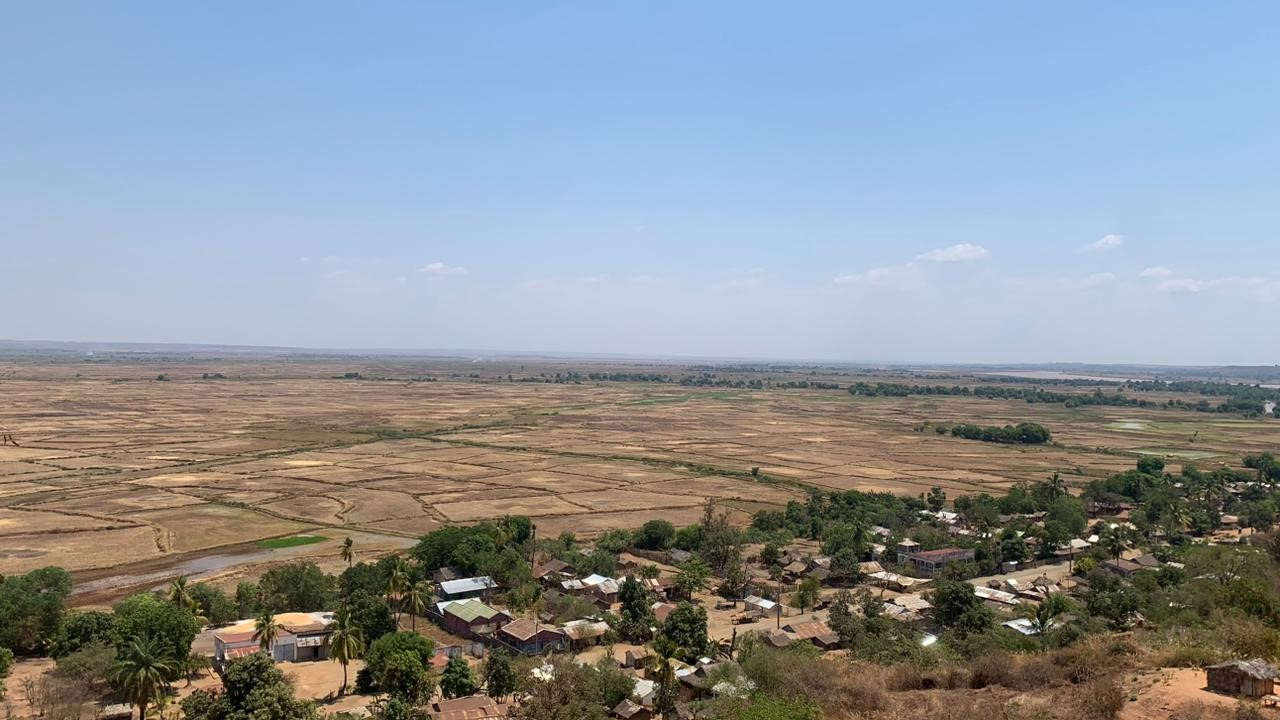
\includegraphics[width=0.75\textwidth]{images/cover-marovoay.jpg}\\[4pt]%
  {\small\itshape Plaine de Marovoay (Copyright Cédrick Rakotoniaina - Projet BETSAKA 2025)}%
  \end{center}%
  \vfill
}
\makeatletter
\@ifpackageloaded{tcolorbox}{}{\usepackage[skins,breakable]{tcolorbox}}
\@ifpackageloaded{fontawesome5}{}{\usepackage{fontawesome5}}
\definecolor{quarto-callout-color}{HTML}{909090}
\definecolor{quarto-callout-note-color}{HTML}{0758E5}
\definecolor{quarto-callout-important-color}{HTML}{CC1914}
\definecolor{quarto-callout-warning-color}{HTML}{EB9113}
\definecolor{quarto-callout-tip-color}{HTML}{00A047}
\definecolor{quarto-callout-caution-color}{HTML}{FC5300}
\definecolor{quarto-callout-color-frame}{HTML}{acacac}
\definecolor{quarto-callout-note-color-frame}{HTML}{4582ec}
\definecolor{quarto-callout-important-color-frame}{HTML}{d9534f}
\definecolor{quarto-callout-warning-color-frame}{HTML}{f0ad4e}
\definecolor{quarto-callout-tip-color-frame}{HTML}{02b875}
\definecolor{quarto-callout-caution-color-frame}{HTML}{fd7e14}
\makeatother
\makeatletter
\@ifpackageloaded{bookmark}{}{\usepackage{bookmark}}
\makeatother
\makeatletter
\@ifpackageloaded{caption}{}{\usepackage{caption}}
\AtBeginDocument{%
\ifdefined\contentsname
  \renewcommand*\contentsname{Table des matières}
\else
  \newcommand\contentsname{Table des matières}
\fi
\ifdefined\listfigurename
  \renewcommand*\listfigurename{Liste des Figures}
\else
  \newcommand\listfigurename{Liste des Figures}
\fi
\ifdefined\listtablename
  \renewcommand*\listtablename{Liste des Tables}
\else
  \newcommand\listtablename{Liste des Tables}
\fi
\ifdefined\figurename
  \renewcommand*\figurename{Figure}
\else
  \newcommand\figurename{Figure}
\fi
\ifdefined\tablename
  \renewcommand*\tablename{Table}
\else
  \newcommand\tablename{Table}
\fi
}
\@ifpackageloaded{float}{}{\usepackage{float}}
\floatstyle{ruled}
\@ifundefined{c@chapter}{\newfloat{codelisting}{h}{lop}}{\newfloat{codelisting}{h}{lop}[chapter]}
\floatname{codelisting}{Listing}
\newcommand*\listoflistings{\listof{codelisting}{Liste des Listings}}
\makeatother
\makeatletter
\makeatother
\makeatletter
\@ifpackageloaded{caption}{}{\usepackage{caption}}
\@ifpackageloaded{subcaption}{}{\usepackage{subcaption}}
\makeatother
\usepackage{bookmark}
\IfFileExists{xurl.sty}{\usepackage{xurl}}{} % add URL line breaks if available
\urlstyle{same}
\hypersetup{
  pdftitle={Campagne 2025 de l'Observatoire rural de Marovoay},
  pdfauthor={Veromanitra Ramizason; Bezaka Rivolala; Thierry Razanakoto; Holimalala Randriamanampisoa; Florent Bédécarrats},
  pdflang={fr},
  colorlinks=true,
  linkcolor={blue},
  filecolor={Maroon},
  citecolor={Blue},
  urlcolor={Blue},
  pdfcreator={LaTeX via pandoc}}


\title{Campagne 2025 de l'Observatoire rural de Marovoay}
\usepackage{etoolbox}
\makeatletter
\providecommand{\subtitle}[1]{% add subtitle to \maketitle
  \apptocmd{\@title}{\par {\large #1 \par}}{}{}
}
\makeatother
\subtitle{Rapport d'enquête}
\author{Veromanitra Ramizason \and Bezaka Rivolala \and Thierry
Razanakoto \and Holimalala Randriamanampisoa \and Florent Bédécarrats}
\date{2026-07-22}
\begin{document}
\maketitle

\renewcommand*\contentsname{Table des matières}
{
\setcounter{tocdepth}{2}
\tableofcontents
}

\bookmarksetup{startatroot}

\chapter*{Introduction}\label{introduction}
\addcontentsline{toc}{chapter}{Introduction}

\markboth{Introduction}{Introduction}

Rapport consolidé d'enquêtes (Version provisoire)

\hfill\break

Les observatoires ruraux constituent un dispositif original de collecte
de données longitudinales mis en place à Madagascar à partir de 1995
afin de documenter les conditions de vie des ménages ruraux et leurs
dynamiques dans le temps. Reposant sur des enquêtes répétées auprès des
mêmes localités, ils combinent des questionnaires ménages standardisés
et des enquêtes communautaires qualitatives, permettant d'articuler
analyse statistique et compréhension fine des contextes locaux.

La campagne 2025 s'inscrit dans cette continuité tout en introduisant
des évolutions méthodologiques. Elle repose sur une articulation étroite
entre enquêtes quantitatives auprès des ménages et enquêtes
communautaires visant à documenter les contextes locaux (pratiques
agricoles, accès aux intrants, sécurité, gouvernance locale). Les
protocoles de terrain intègrent également des exigences renforcées en
matière d'éthique, de consentement éclairé et d'interaction avec les
autorités locales à différents niveaux administratifs.

Dans le cadre du projet BETSAKA, ce dispositif est aujourd'hui réactivé
afin d'analyser les effets de long terme des politiques de conservation,
en particulier des aires protégées, sur les conditions de vie des
populations et les dynamiques environnementales. Le projet s'appuie sur
une combinaison de données historiques, d'images satellitaires et de
nouvelles enquêtes de terrain pour étudier conjointement déforestation,
feux et trajectoires socio-économiques.

Ce document présente le traitement et l'analyse des données de
l'observatoire rural de Marovoay pour la campagne 2025. La période de
référence s'étend d'octobre 2024 à septembre 2025. Ces données ont été
récoltées afin d'étudier l'évaluation d'impact de la conservation sur
les conditions de vie des ménages aux alentours de l'aire protégée
d'Ankarafantsika.

Les chapitres suivants détaillent successivement les principes
méthodologiques des observatoires, l'organisation de la collecte, les
instruments d'enquête et les choix opérés pour la campagne 2025.
L'objectif est double : assurer la transparence du dispositif et
faciliter la réutilisation des données, tout en rendant explicites les
arbitrages méthodologiques qui conditionnent leur interprétation.

\bookmarksetup{startatroot}

\chapter{Description de l'enquête}\label{description-de-lenquuxeate}

\section{Contexte et objectifs}\label{contexte-et-objectifs}

Les Observatoires Ruraux (OR) de Madagascar sont un dispositif d'enquête
longitudinale auprès de ménages ruraux, mis en place à partir de 1995
dans le cadre du réseau des observatoires ruraux coordonné par l'IRD et
l'INSTAT, puis le Ministère en charge de l'Agriculture.

\begin{itemize}
\tightlist
\item
  \textbf{Marovoay} constitue le deuxième pôle rizicole du pays, avec
  une production reposant sur l'irrigation par les eaux du fleuve
  Betsiboka. L'observatoire de Marovoay est situé dans la plaine
  alluviale du fleuve Betsiboka, dans le district de Marovoay de la
  région Boeny, au nord-ouest de Madagascar. La zone d'enquête
  s'organise autour de quatre fokontany --- Ampijoroa et Maroala sur la
  rive gauche, Bepako et Madiromiongana sur la rive droite --- séparés
  par le fleuve. La proximité du Parc national d'Ankarafantsika, dont
  les limites ont été étendues en 2002, confère à cette zone un intérêt
  particulier pour l'étude des interactions entre conservation et
  développement rural. L'économie locale repose principalement sur la
  riziculture irriguée, complétée par l'élevage bovin et les cultures de
  rente.
\end{itemize}

Les principales modifications du questionnaire concernent :

\begin{itemize}
\item
  la suppression du module dédié aux dépenses (D), qui était très long à
  administrer et qui avait peu été exploité dans le passé ;
\item
  l'introduction de nouveaux modules sur les évènements climatiques
  extrêmes (CC), la sécurité alimentaire (SA-SSA), feux (S), le rapport
  des ménages ruraux avec l'environnement (RM-UM-AP).
\end{itemize}

La période de référence couvre les douze mois précédant l'interview,
soit du 1\textsuperscript{er} octobre 2024 au 30 septembre 2025.

\section{Méthodologie}\label{muxe9thodologie}

L'enquête reprend le protocole des campagnes antérieures des
Observatoires Ruraux. Le questionnaire ménage couvre l'ensemble des
dimensions socio-économiques : démographie, habitat, activités agricoles
et non agricoles, foncier, revenus, sécurité alimentaire, environnement
et événements climatiques.

Les unités d'observation sont les ménages résidant dans les hameaux
échantillonnés. L'échantillon de 2025 vise à reconstituer autant que
possible le panel de ménages suivis lors des campagnes précédentes,
complété par de nouveaux ménages en remplacement de ceux ayant quitté la
zone ou disparus.

Avant le déploiement sur le terrain, Les enquêteurs ont été formés par
les superviseurs selon une approche de formation en cascade. La saisie
des données a été réalisée directement sur le terrain à l'aide de
masques de saisie dédiés permettant un gain de temps grâce à la
disponibilité immédiate des données pour l'analyse, une détection
précoce des incohérences facilitant leur nettoyage, ainsi qu'un retour
possible dans les ménages en cas de besoin pendant la phase de collecte.

\begin{tcolorbox}[enhanced jigsaw, arc=.35mm, bottomrule=.15mm, bottomtitle=1mm, breakable, colback=white, colbacktitle=quarto-callout-note-color!10!white, colframe=quarto-callout-note-color-frame, coltitle=black, left=2mm, leftrule=.75mm, opacityback=0, opacitybacktitle=0.6, rightrule=.15mm, title=\textcolor{quarto-callout-note-color}{\faInfo}\hspace{0.5em}{Note}, titlerule=0mm, toprule=.15mm, toptitle=1mm]

Le protocole éthique de l'enquête a fait l'objet d'une approbation. Il
est présenté en annexe du rapport.

\end{tcolorbox}

\section{Localisation des sites
enquêtés}\label{localisation-des-sites-enquuxeatuxe9s}

Les coordonnées GPS des hameaux enquêtés ont été relevées lors de la
campagne. La carte ci-dessous présente la localisation approximative de
chaque fokontany, calculée comme le centroïde des hameaux qui le
composent.

\begin{figure}[H]

\caption{Localisation approximative des fokontany enquêtés (centroïde
des hameaux)}

{\centering \pandocbounded{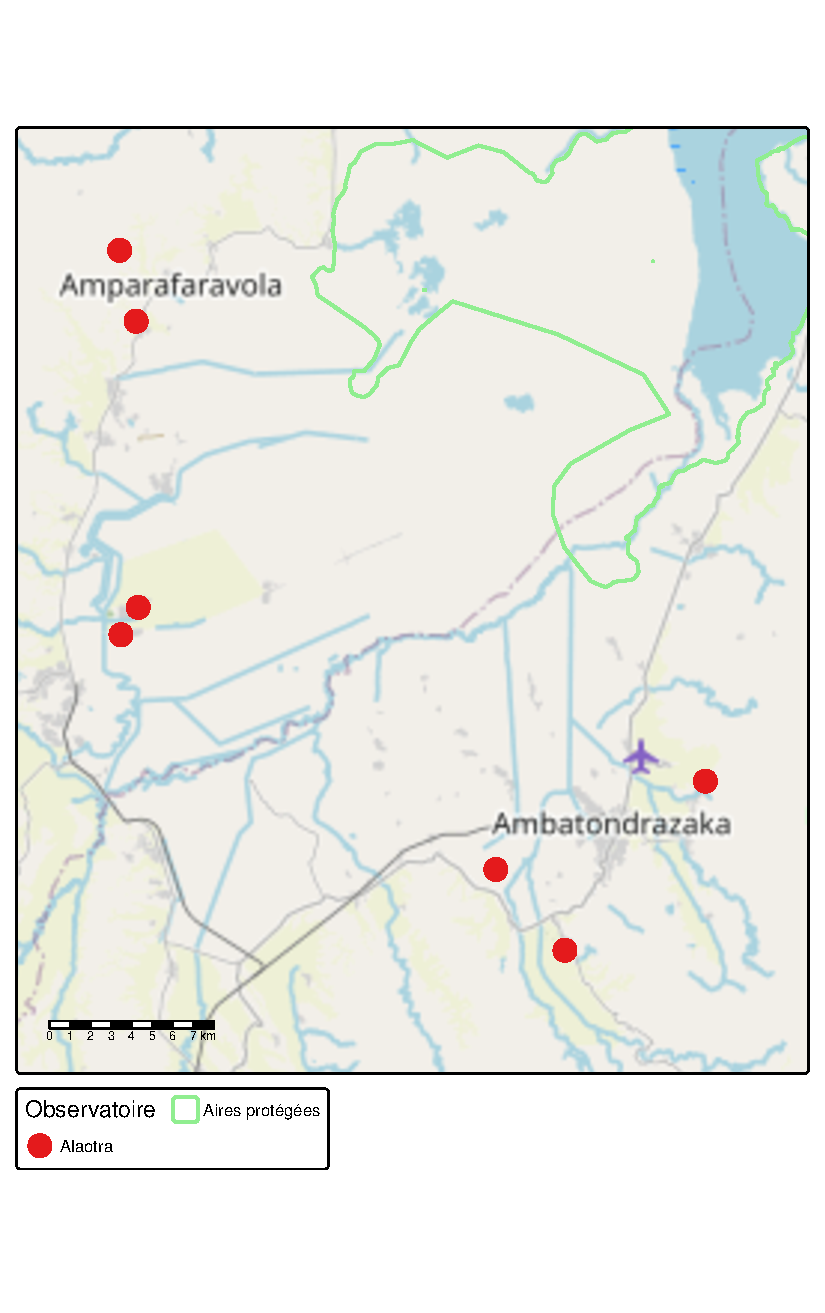
\includegraphics[keepaspectratio]{01_description_files/figure-pdf/carte_sites-1.pdf}}

}

\end{figure}%

\section{Ménages enquêtés}\label{muxe9nages-enquuxeatuxe9s}

A Marovoay, 519 ménages ont été enquêtés pour 2 297 individus.

Voir Table~\ref{tbl-men-obs}.

\begin{table}

\caption{\label{tbl-men-obs}Répartition des ménages et des individus
selon les observatoires}

\centering{

}

\end{table}%

\subsection{Dénombrement et taux de
sondage}\label{duxe9nombrement-et-taux-de-sondage}

Le dénombrement préalable à l'enquête a recensé l'ensemble des ménages
résidant dans les hameaux échantillonnés. Le
Table~\ref{tbl-denombrement} confronte le nombre de ménages dénombrés au
nombre de ménages effectivement enquêtés. Bien que le nombre de ménages
enquêtés soit similaire, l'effort d'échantillonnage est 2.5 fois plus
intense à Marovoay avec plus d'un ménage sur 5 interrogé. Cela
s'explique par une population de base beaucoup plus vaste dans les
hameaux sélectionnés de l'Alaotra (un ménage enqueté sur 12 parmi ceux
recensés dans les hameaux). Le taux de sondage global est de l'ordre de
18 \%.

\textbf{Marovoay :} 2 506 ménages dénombrés pour un taux de sondage de
20.7 \%.

\begin{table}

\caption{\label{tbl-denombrement}Dénombrement et taux de sondage par
observatoire}

\centering{

}

\end{table}%

\subsection{Répartition par hameau}\label{ruxe9partition-par-hameau}

Le Table~\ref{tbl-men-hameau} détaille le nombre de ménages enquêtés
dans chacun des hameaux, regroupés par site au sein de chaque
observatoire. La structure spatiale de l'échantillon à l'Alaotra est
plus fragmentée (8 sites contre 4 à Marovoay), reflétant la diversité
des contextes autour de ces deux observatoires.

Marovoay : La répartition est plus concentrée sur 4 sites avec une
prédominance d'Ampijoroa (27.6 \%) et de Madiromiongana (26.4 \%).

\begin{table}

\caption{\label{tbl-men-hameau}Répartition des ménages enquêtés par
hameau}

\centering{

\fontsize{12.0pt}{14.4pt}\selectfont
\begin{tabular*}{\linewidth}{@{\extracolsep{\fill}}lrr}
\toprule
Hameau & Ménages & \% obs. \\ 
\midrule\addlinespace[2.5pt]
\multicolumn{3}{l}{{\bfseries {Alaotra}}} \\[2.5pt] 
\midrule\addlinespace[2.5pt]
Avaradrano & 90 & 17.8 \\ 
Feramanga Atsimo & 89 & 17.6 \\ 
Mangabe & 73 & 14.4 \\ 
Ambatomanga & 68 & 13.4 \\ 
Ambodivoara & 58 & 11.4 \\ 
Ambohidrony & 52 & 10.3 \\ 
Analamiranga & 46 & 9.1 \\ 
Ambatoharanana & 31 & 6.1 \\ 
{\bfseries {Ensemble}} & {\bfseries {507}} & {\bfseries {100.0}} \\ 
\midrule\addlinespace[2.5pt]
\multicolumn{3}{l}{{\bfseries {Marovoay}}} \\[2.5pt] 
\midrule\addlinespace[2.5pt]
Ampijoroa & 143 & 27.6 \\ 
Madiromiongana & 137 & 26.4 \\ 
Bepako & 123 & 23.7 \\ 
Maroala & 116 & 22.4 \\ 
{\bfseries {Ensemble}} & {\bfseries {519}} & {\bfseries {100.0}} \\ 
\bottomrule
\end{tabular*}
\begin{minipage}{\linewidth}
\textbf{Source : Enquête auprès des OR 2025}\\
\end{minipage}

}

\end{table}%

\section{Déroulement de l'enquête}\label{duxe9roulement-de-lenquuxeate}

Les entretiens se sont déroulés entre début octobre et mi-novembre 2025.
Le Figure~\ref{fig-chronogramme} présente l'évolution cumulée du nombre
d'entretiens réalisés à partir du 1\textsuperscript{er} octobre 2025.

\begin{figure}

\caption{\label{fig-chronogramme}Fréquences cumulées des entretiens par
observatoire (à partir du 1er octobre 2025)}

\centering{

\pandocbounded{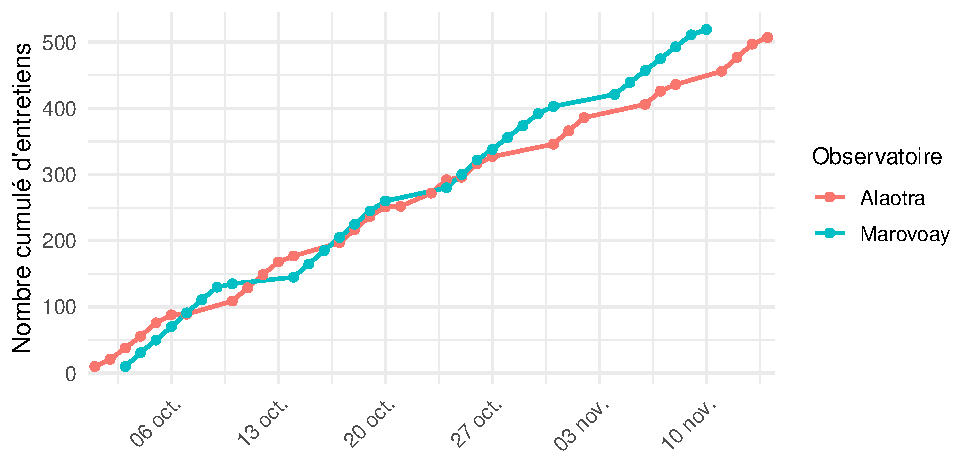
\includegraphics[keepaspectratio]{01_description_files/figure-pdf/fig-chronogramme-1.pdf}}

}

\end{figure}%

Les enquêteurs ont réalisé un nombre de questionnaires quotidien très
stable sans interruption majeure ni ralentissement.

\begin{table}

\caption{\label{tbl-periode}Période de collecte par observatoire}

\centering{

}

\end{table}%

L'enquête a mobilisé 20 enquêteurs (10 par observatoire), encadrés par 6
superviseurs (3 par observatoire). La saisie des questionnaires a été
assurée par 4 opérateurs.

\bookmarksetup{startatroot}

\chapter{Caractéristiques socio-démographiques des
ménages}\label{caractuxe9ristiques-socio-duxe9mographiques-des-muxe9nages}

Le ménage est l'unité de base de l'enquête. Cette section décrit la
composition des ménages, les caractéristiques des chefs de ménage et de
leurs membres, ainsi que l'évolution de ces indicateurs.

À Marovoay, la structure des ménages est marquée par l'hétérogénéité des
stratégies économiques et des structures familiales. La proximité de la
ville de Marovoay et de la route nationale RN4 reliant Antananarivo à
Mahajanga facilite les échanges et influence les activités non agricoles
des ménages.

\section{Description des ménages}\label{description-des-muxe9nages}

\subsection{Taille des ménages}\label{taille-des-muxe9nages}

Le ménage est un ensemble de personnes avec ou sans lien de parenté,
vivant sous le même toit ou dans la même concession, prenant leur repas
ensemble ou par petits groupes, mettant une partie ou la totalité de
leurs revenus en commun pour la bonne marche du groupe.

A Marovoay, on a recensé 2297 individus répartis dans 519 ménages. La
taille moyenne des ménages s'établit à 4.4 personnes.

\begin{figure}[H]

\caption{Taille moyenne des ménages par hameau selon les observatoires}

{\centering \pandocbounded{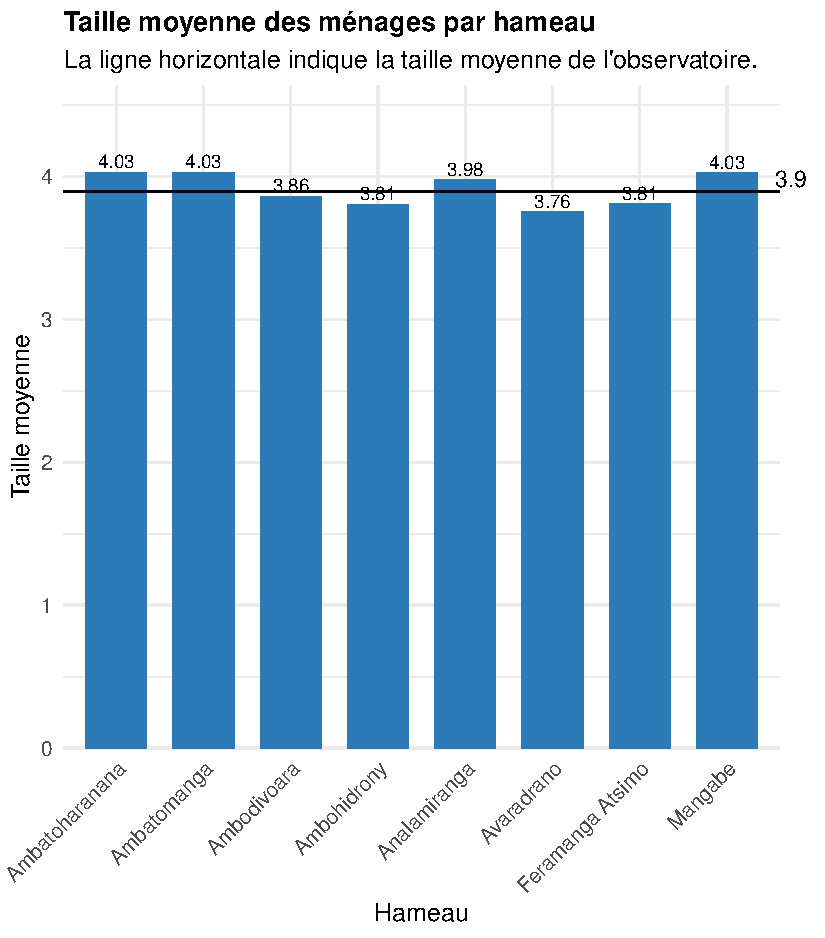
\includegraphics[keepaspectratio]{02_structure_menages_files/figure-pdf/fig_men_hameau-1.pdf}}

}

\end{figure}%

\subsection{Structure par âge}\label{structure-par-uxe2ge}

La structure démographique des ménages enquêtés révèle une population
jeune. Cette distribution, caractéristique des populations rurales
malgaches, implique un fort taux de dépendance.

\subsubsection{Au niveau des
observatoires}\label{au-niveau-des-observatoires}

La population est extrêmement jeune, avec une base de pyramide (0-10
ans) représentant près de 30 \% des effectifs dans les deux zones.
Marovoay présente un taux de dépendance des jeunes plus élevé
qu'Alaotra.

A Marovoay, 40.7 \% des individus ont moins de 15 ans, signe d'une
population en croissance rapide. La population en âge de travailler
(15--64 ans) représente 54.7 \%, tandis que les personnes de 65 ans et
plus ne constituent que 4.6 \%. Cette structure démographique,
caractérisée par une base large et un sommet étroit, est caractéristique
des populations rurales malgaches et traduit un taux de dépendance
élevé.

\begin{figure}[H]

\caption{Pyramide des âges des membres des ménages enquêtés par
observatoire}

{\centering \pandocbounded{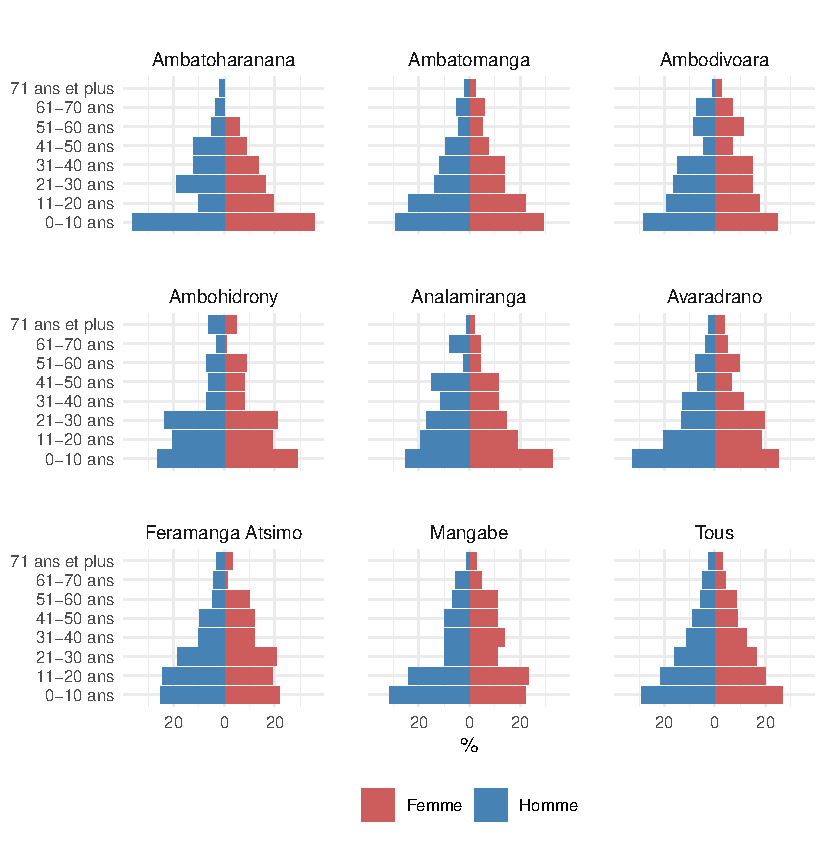
\includegraphics[keepaspectratio]{02_structure_menages_files/figure-pdf/fig_pyramide-1.pdf}}

}

\end{figure}%

\subsection{Origine des Chefs de Ménage et
conjoints}\label{origine-des-chefs-de-muxe9nage-et-conjoints}

L'origine géographique des chefs de ménage (CM) et de leurs conjoints
renseigne sur les dynamiques migratoires et le degré d'ancrage local des
familles. La classification distingue les \emph{tompon-tany}
(autochtones), les \emph{zana-tany} (nés sur place de parents migrants),
les \emph{valivotaka} (migrants installés durablement) et les
\emph{mpihavy} (arrivants récents).

À Marovoay, l'équilibre entre \emph{tompon-tany} (39 \%) et
\emph{zana-tany} (39.4 \%)varie selon les localités. La proportion de
\emph{valivotaka} et \emph{mpihavy} reflète l'attractivité des zones
rizicoles pour les migrants des régions voisines. Les raisons sociales
(en particulier le mariage) dépassent largement les motivations
économiques comme facteur d'installation.

\pandocbounded{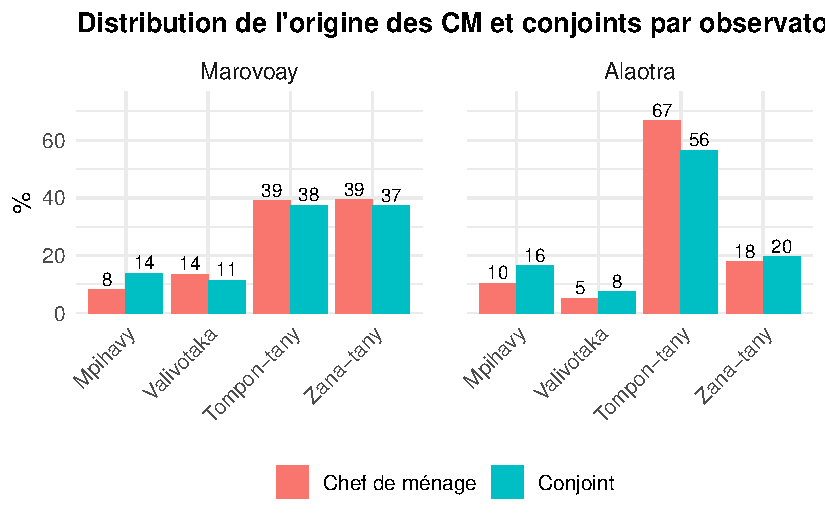
\includegraphics[keepaspectratio]{02_structure_menages_files/figure-pdf/fig_origine-1.pdf}}

\subsection{Raison d'installation}\label{raison-dinstallation}

Les raisons d'installation des CM et conjoints non originaires du lieu
éclairent les motivations migratoires. Elles distinguent notamment les
installations liées au mariage de celles motivées par les opportunités
économiques (travail agricole ou non agricole).

À Marovoay, les raisons sociales représentent également le principal
motif d'implantation, avec 89.6\% des conjoints et 83.8\% des chefs de
ménage concernés. Les motivations économiques, associées au travail et à
l'accès aux ressources, occupent une place plus importante chez les
chefs de ménage, où elles atteignent 15.6\%, contre 9.8\% chez les
conjoints.

\pandocbounded{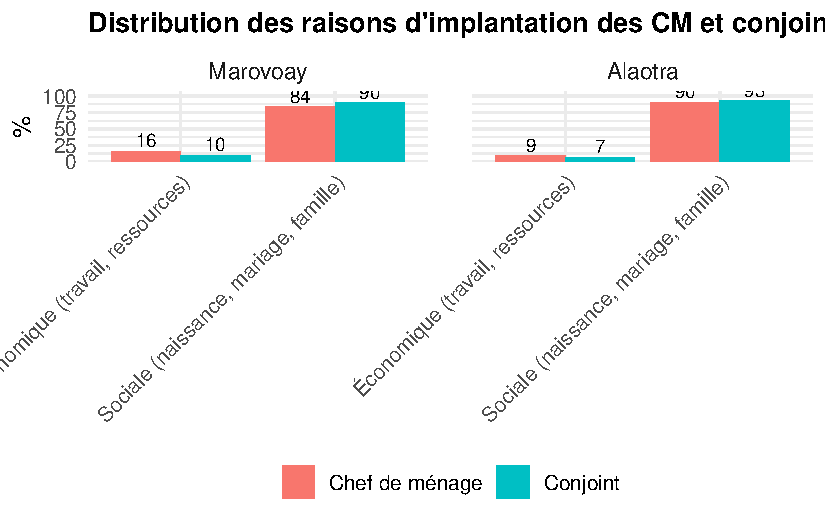
\includegraphics[keepaspectratio]{02_structure_menages_files/figure-pdf/fig_raison-1.pdf}}

\section{Caractéristiques des chefs de
ménages}\label{caractuxe9ristiques-des-chefs-de-muxe9nages}

Cette section analyse le profil des chefs de ménage dans les deux
observatoires, en examinant notamment leurs caractéristiques
socio-démographiques, leur niveau d'éducation, leur alphabétisation,
ainsi que leurs activités principales.

\subsection{Caractéristiques
socio-démographiques}\label{caractuxe9ristiques-socio-duxe9mographiques}

Le profil des chefs de ménage (CM) est décrit ci-dessous.

A Marovoay, 78 \% des CM sont des hommes, soit 22 \% de ménages dirigés
par des femmes. L'âge moyen des CM est de 46.1 ans. Sur le plan
conjugal, 73 \% des CM vivent en couple (mariés ou en concubinage).

\begin{table}
\caption*{
{\large Caractéristiques des chefs de ménage\textsuperscript{\textit{1}}}
} 
\fontsize{12.0pt}{14.4pt}\selectfont
\begin{tabular*}{\linewidth}{@{\extracolsep{\fill}}lr}
\toprule
{\bfseries {Catégorie}} & {\bfseries {Marovoay}} \\ 
\midrule\addlinespace[2.5pt]
\multicolumn{2}{l}{{\bfseries {Sexe}}} \\[2.5pt] 
\midrule\addlinespace[2.5pt]
Femme & 22\% \\ 
Homme & 78\% \\ 
\midrule\addlinespace[2.5pt]
\multicolumn{2}{l}{{\bfseries {Âge}}} \\[2.5pt] 
\midrule\addlinespace[2.5pt]
Minimum & 18 \\ 
Mode & 36 \\ 
Médiane & 45 \\ 
Moyenne & 46 \\ 
Maximum & 96 \\ 
\bottomrule
\end{tabular*}
\begin{minipage}{\linewidth}
\textsuperscript{\textit{1}}Sexe : effectifs et pourcentages. Âge : statistiques descriptives.\\
\textbf{Source : Enquête auprès des OR 2025}\\
\end{minipage}
\end{table}

\begin{figure}[H]

\caption{Statut matrimonial des chefs de ménage}

{\centering \pandocbounded{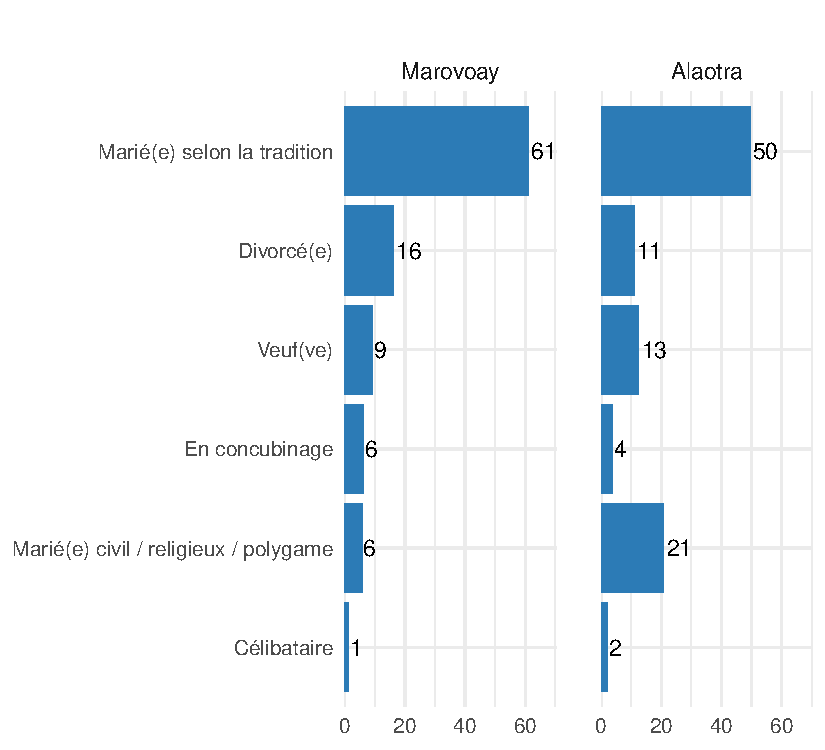
\includegraphics[keepaspectratio]{02_structure_menages_files/figure-pdf/fig_cm_statut-1.pdf}}

}

\end{figure}%

\subsection{Niveau d'éducation}\label{niveau-duxe9ducation}

Le niveau d'éducation des chefs de ménage constitue un déterminant
majeur de la capacité d'adaptation et de la vulnérabilité des ménages
ruraux. L'analyse croisée par sexe met en évidence des disparités
supplémentaires.

\subsubsection{Niveau d'éducation du Chef de
ménage}\label{niveau-duxe9ducation-du-chef-de-muxe9nage}

À Marovoay, la structure éducative est plus hétérogène avec une part de
non-scolarisation de 13.9 \%. Si le niveau primaire demeure la référence
pour 51.8 \% des chefs, on note paradoxalement une insertion plus forte
dans le premier cycle secondaire qui atteint 25.0 \%. Ces chiffres
traduisent une disparité interne plus marquée dans l'accès aux cycles
d'études au sein de cet observatoire.

\begin{figure}[H]

\caption{Niveau d'éducation des chefs de ménage}

{\centering \pandocbounded{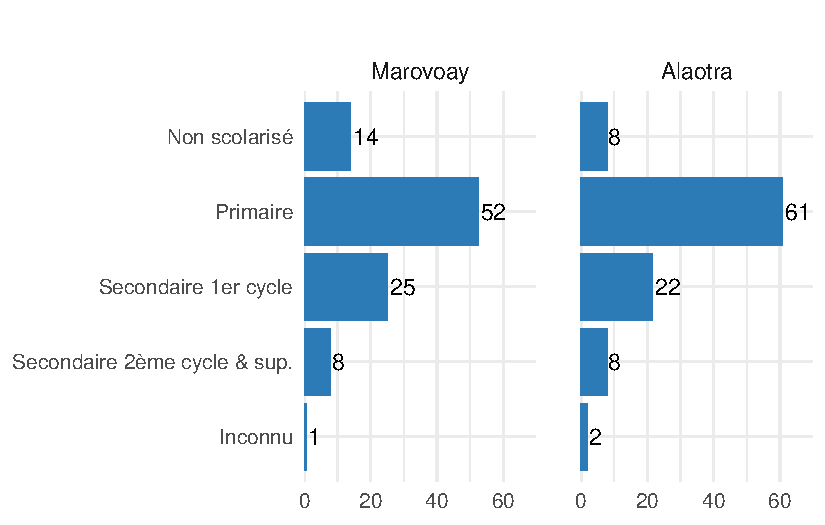
\includegraphics[keepaspectratio]{02_structure_menages_files/figure-pdf/fig_cm_educ-1.pdf}}

}

\end{figure}%

\subsubsection{Niveau d'éducation des chefs de ménages par
sexe}\label{niveau-duxe9ducation-des-chefs-de-muxe9nages-par-sexe}

Il existe un fossé de genre persistant pour l'accès aux études longues :
les hommes chefs de ménage ont environ deux fois plus de chances
d'atteindre le second cycle du secondaire ou le niveau supérieur par
rapport aux femmes, et ce, dans les deux observatoires. Le niveau
``Primaire'' reste le socle commun le plus fréquent pour les deux sexes,
oscillant entre 49 \% et 64 \% selon les catégories.

A Marovoay, les femmes chefs de ménage présentent des taux d'instruction
nettement plus faibles que les hommes, ce qui accentue leur
vulnérabilité socio-économique. Les hommes sont deux fois plus nombreux
(9.1 \%) que les femmes (4.4 \%) à atteindre les cycles d'études les
plus longs. Si les femmes de Marovoay accèdent plus souvent à l'école
que les hommes (moins de non-scolarisées et plus de niveau primaire avec
61.4 \%), elles sont plus précocement limitées dans leur progression
vers les niveaux secondaires et supérieurs par rapport à leurs
homologues masculins. Contrairement à la tendance habituelle, le taux de
non-scolarisation est plus élevé chez les chefs de ménage hommes (14.6
\%) que chez les femmes (11.4 \%).

\begin{figure}[H]

\caption{Niveau d'éducation des CM par sexe}

{\centering \pandocbounded{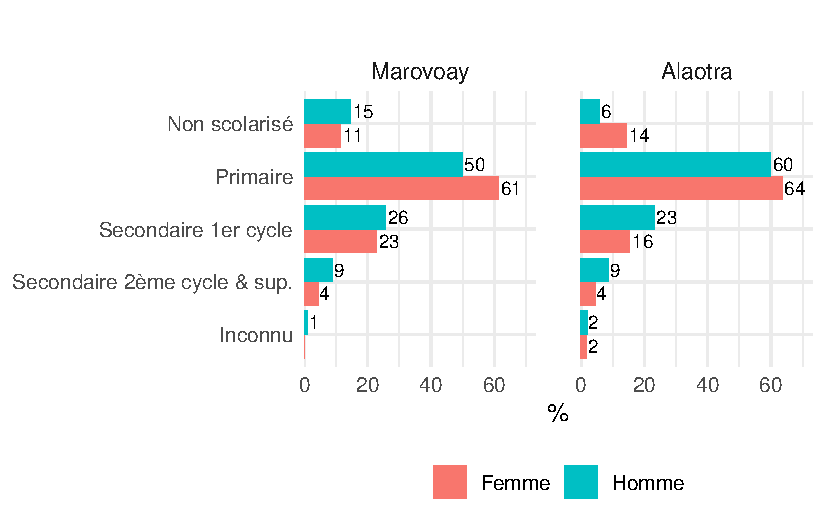
\includegraphics[keepaspectratio]{02_structure_menages_files/figure-pdf/fig_cm_educ_sex-1.pdf}}

}

\end{figure}%

\subsection{Alphabétisation des chefs de
ménage}\label{alphabuxe9tisation-des-chefs-de-muxe9nage}

L'aptitude à lire et écrire conditionne l'accès à l'information, aux
services publics et aux opportunités économiques. Les sections suivantes
détaillent les compétences en lecture et en écriture séparément, en
distinguant trois niveaux : lecture/écriture aisée, avec effort, ou
absente.

\subsubsection{Savoir lire}\label{savoir-lire}

L'aptitude à la lecture est nettement supérieure dans le bassin de
l'Alaotra. À Marovoay, un Chef de ménage sur 5 ne sait pas lire du tout.

A Marovoay, 74 \% des CM savent lire aisément.

À Marovoay, les niveaux d'aptitude à la lecture sont relativement
similaires entre les sexes, avec 74.6\% des femmes et 73.8\% des hommes
sachant lire. À l'inverse, les proportions de chefs de ménage ne sachant
pas lire demeurent importantes, atteignant 20.5\% chez les hommes et
18.4\% chez les femmes.

La lecture avec difficulté concerne une faible proportion des chefs de
ménage quelque soit leur genre.

\begin{figure}[H]

\caption{Aptitude à la lecture des CM selon le sexe}

{\centering \pandocbounded{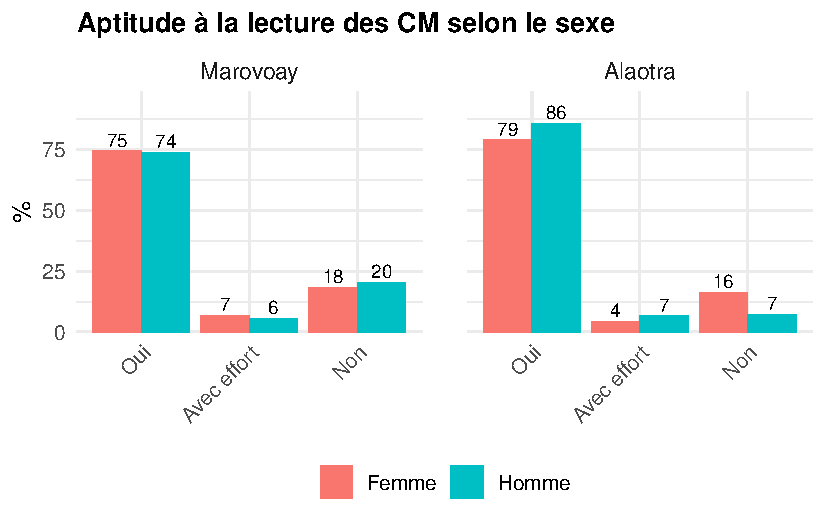
\includegraphics[keepaspectratio]{02_structure_menages_files/figure-pdf/fig_cm_read_sex-1.pdf}}

}

\end{figure}%

\subsubsection{Savoir écrire}\label{savoir-uxe9crire}

On observe une corrélation presque parfaite entre lecture et écriture
dans les deux zones.

À Marovoay, la proportion de chefs de ménage rencontrant des obstacles
face à l'écrit est nettement plus marquée, atteignant 27.1 \%. Ce groupe
se compose de 20.4 \% de personnes incapables d'écrire et de 6.7 \% de
personnes le faisant avec effort.

À Marovoay, les niveaux d'aptitude à l'écriture sont relativement
proches entre les sexes, avec 73.7\% des femmes et 72.6\% des hommes
sachant écrire. Par ailleurs, les proportions de chefs de ménage ne
sachant pas écrire demeurent importantes, atteignant 20.7\% chez les
hommes et 19.3\% chez les femmes.

Les chefs de ménage capables d'écrire avec difficulté restent peu
nombreux.

\begin{figure}[H]

\caption{Aptitude à l'écriture des CM selon le sexe}

{\centering \pandocbounded{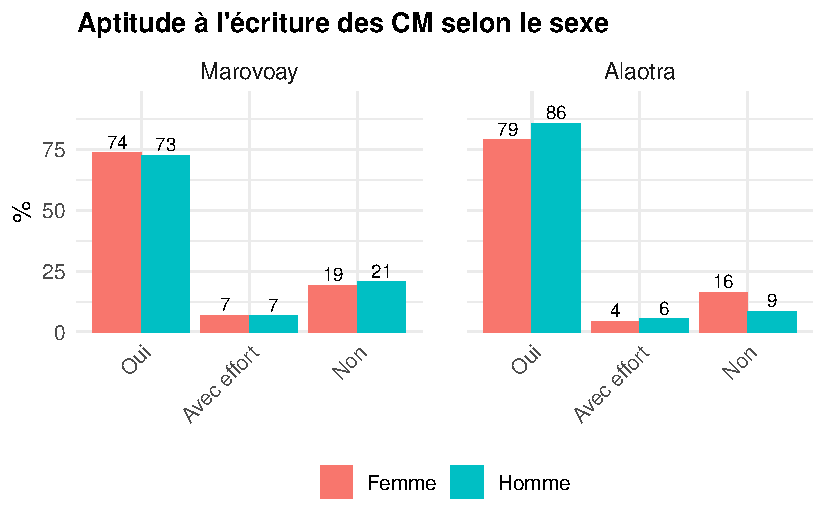
\includegraphics[keepaspectratio]{02_structure_menages_files/figure-pdf/fig_cm_write_sex-1.pdf}}

}

\end{figure}%

\subsection{Activités principales des Chefs de
ménage}\label{activituxe9s-principales-des-chefs-de-muxe9nage}

L'activité économique principale des chefs de ménage traduit la
structure productive de chaque observatoire. Les activités sont
regroupées en catégories sectorielles inspirées de la CITI Rév. 4 afin
de garantir un effectif suffisant dans chaque classe et de préserver la
confidentialité statistique.

L'activité de «Cultivateur exploitant» occupe une place importante dans
les deux OR. Les proportions des ouvriers agricoles indiquent un recours
plus fréquent au salariat.

A Marovoay, l'activité dominante est « Cultivateur exploitant » (58.6 \%
des CM). On note une part significative d'ouvriers agricoles qui
comptent pour 18.3 \% des CM. L'agriculture constitue le socle
économique des ménages, les cultivateurs exploitants représentant la
majorité des chefs de ménage. Le commerce et la restauration,
l'artisanat, le BTP et le transport, ainsi que l'élevage et la pêche
complètent le panorama des activités.Le commerce et la restauration
représentent l'activité principale de 7.3 \% des CM, suivi par les
métiers de l'artisanat, du BTP et du transport qui concernent 6.7 \%
d'entre eux

\begin{figure}

\caption{\label{fig-cm-act}Activités principales des chefs de ménages}

\centering{

\pandocbounded{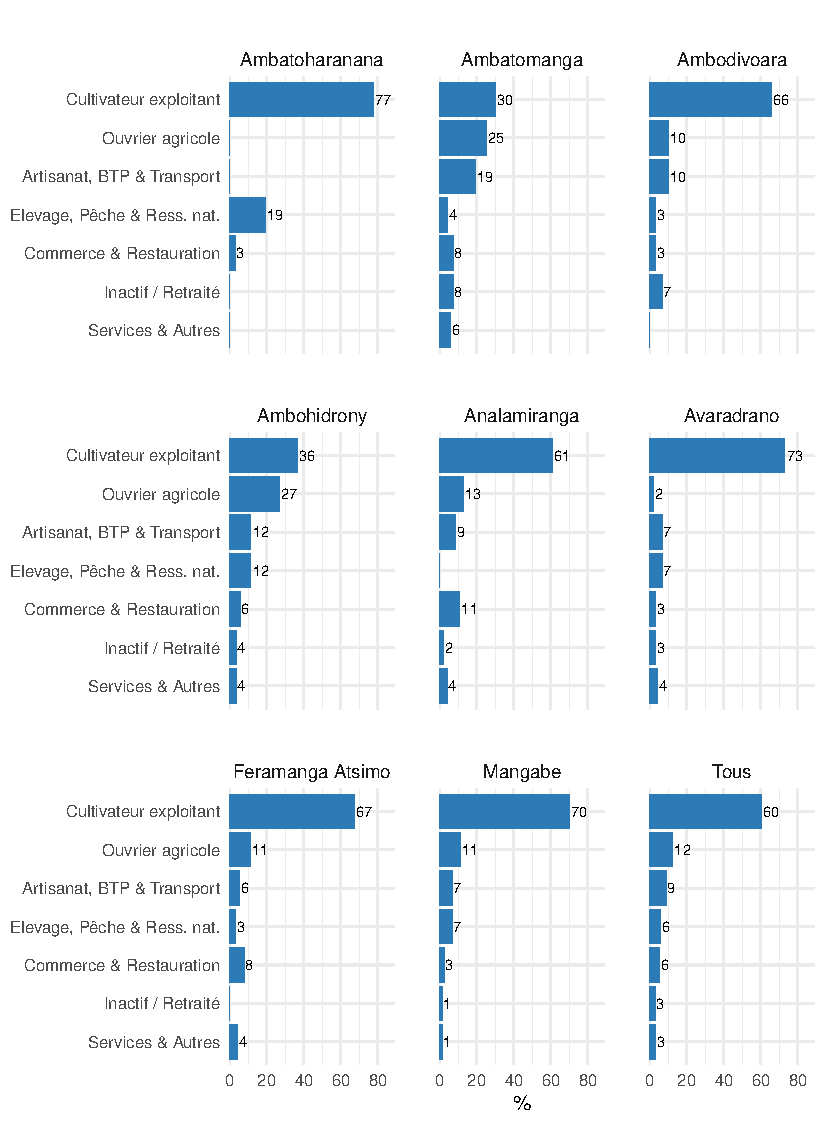
\includegraphics[keepaspectratio]{02_structure_menages_files/figure-pdf/fig-cm-act-1.pdf}}

}

\end{figure}%

\subsubsection{Activités principales des CM par
sexe}\label{activituxe9s-principales-des-cm-par-sexe}

Cette section examine les activités principales des chefs de ménage
selon leur genre au sein des deux observatoires.

À Marovoay, la différenciation des activités selon le sexe est marquée.
Les hommes sont majoritairement cultivateurs exploitants : 65.9 \% des
hommes CM sont cultivateurs exploitants, alors que seulement 32.5 \% des
femmes occupent ce statut. Un recours massif au salariat agricole est
constaté chez les femmes CM avec 30.7 \% contre 14.8 \% pour les hommes.
Par ailleurs, les femmes sont davantage présentes dans le commerce et la
restauration.

\begin{figure}[H]

\caption{Activités principales des CM par observatoire et sexe}

{\centering \pandocbounded{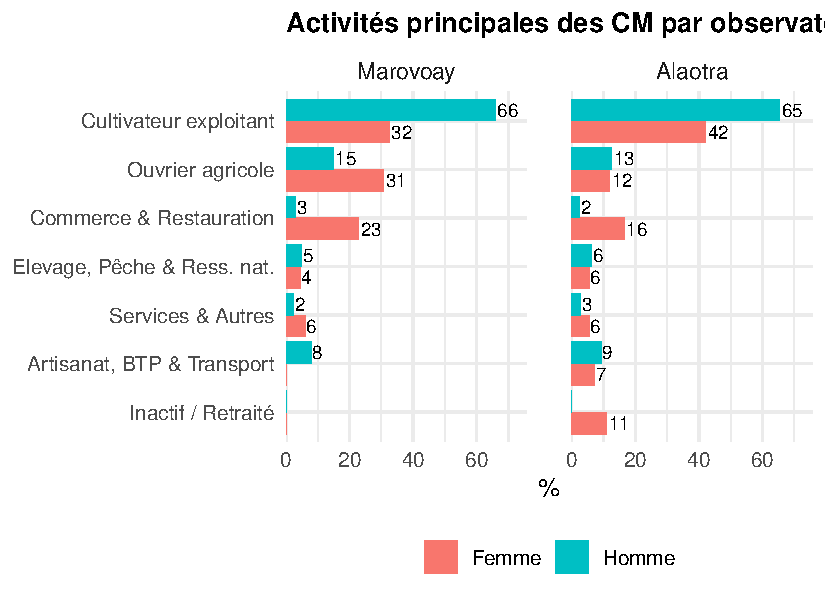
\includegraphics[keepaspectratio]{02_structure_menages_files/figure-pdf/fig_cm_act_sex-1.pdf}}

}

\end{figure}%

\section{Caractéristiques des autres membres de
ménages}\label{caractuxe9ristiques-des-autres-membres-de-muxe9nages}

Les autres membres du ménage (conjoints, enfants, dépendants)
constituent la majorité de la population recensée. Leur profil
démographique, éducatif et économique complète celui des chefs de ménage
et permet de dresser un portrait plus complet du capital humain des
familles rurales.

\subsection{Caractéristiques
socio-démographiques}\label{caractuxe9ristiques-socio-duxe9mographiques-1}

Cette section analyse les caractéristiques des conjoints, enfants et
dépendants, qui forment la majorité des membres du ménage autres que le
CM.

À Marovoay, les autres membres du ménage forment une population
majoritairement féminine et jeune avec 58.8 \% de femmes et 41.1 \%
d'hommes.Les indicateurs d'âge révèlent un profil démographique
caractéristique des populations rurales en croissance. La population
affiche une grande jeunesse avec un âge moyen de 18 ans et un âge médian
de 14 ans. Pour les membres de 12 ans et plus, la prédominance des
mariages selon la tradition (40.3 \%) et du célibat (41.3 \%) témoigne
du maintien des pratiques matrimoniales coutumières.

\begin{figure}[H]

\caption{Statut matrimonial des autres membres (12 ans et plus)}

{\centering \pandocbounded{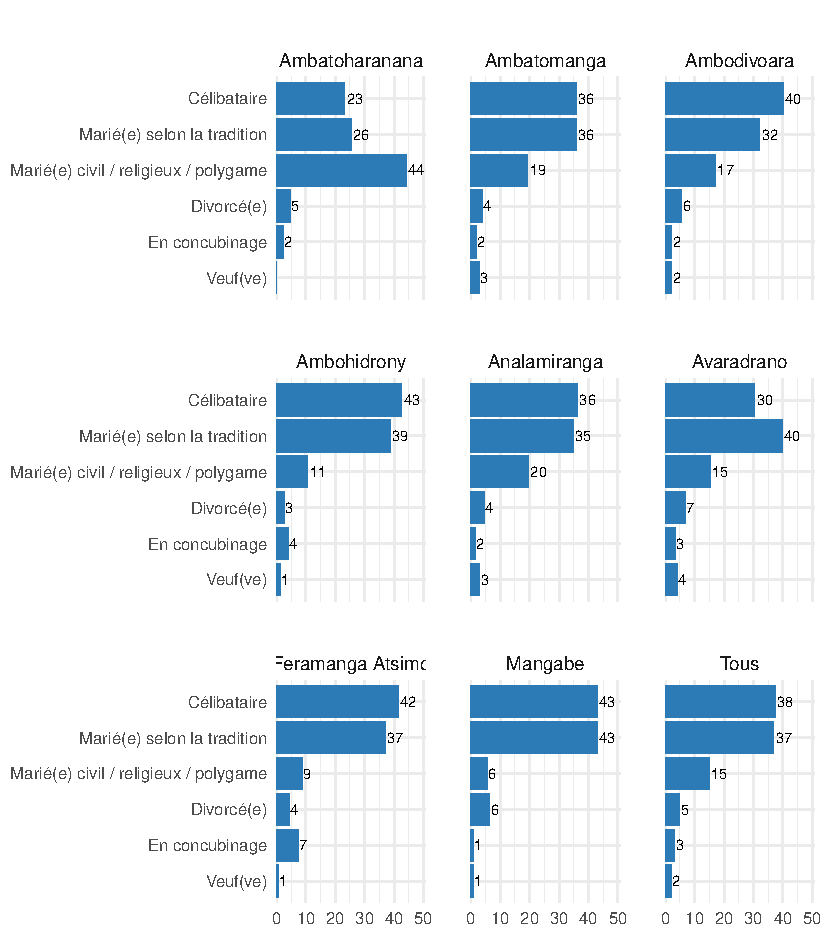
\includegraphics[keepaspectratio]{02_structure_menages_files/figure-pdf/fig_other_statut-1.pdf}}

}

\end{figure}%

\subsection{Éducation et
scolarisation}\label{uxe9ducation-et-scolarisation}

Le niveau d'éducation des autres membres de ménage complète le portrait
éducatif des familles. Les disparités entre sexes et entre observatoires
donnent un aperçu des inégalités d'accès à l'éducation.

\subsubsection{Niveau d'éducation des autres
membres}\label{niveau-duxe9ducation-des-autres-membres}

L'analyse du niveau d'éducation des membres des ménages révèle des
disparités importantes entre les deux bassins rizicoles notamment en
termes d'accès initial à l'école et de poursuite des cycles d'études.

À Marovoay, le niveau primaire reste majoritaire avec 48.0 \% des
membres. Cependant, l'observatoire affiche un retard structurel d'accès
à l'école avec un taux de non-scolarisation s'élevant à 27.4 \%.
Concernant 20.8\% des individus, l'accès aux niveaux secondaire et
supérieur y est plus limité concernant 20.8 \% des individus.

\begin{figure}[H]

\caption{Niveau d'éducation des autres membres}

{\centering \pandocbounded{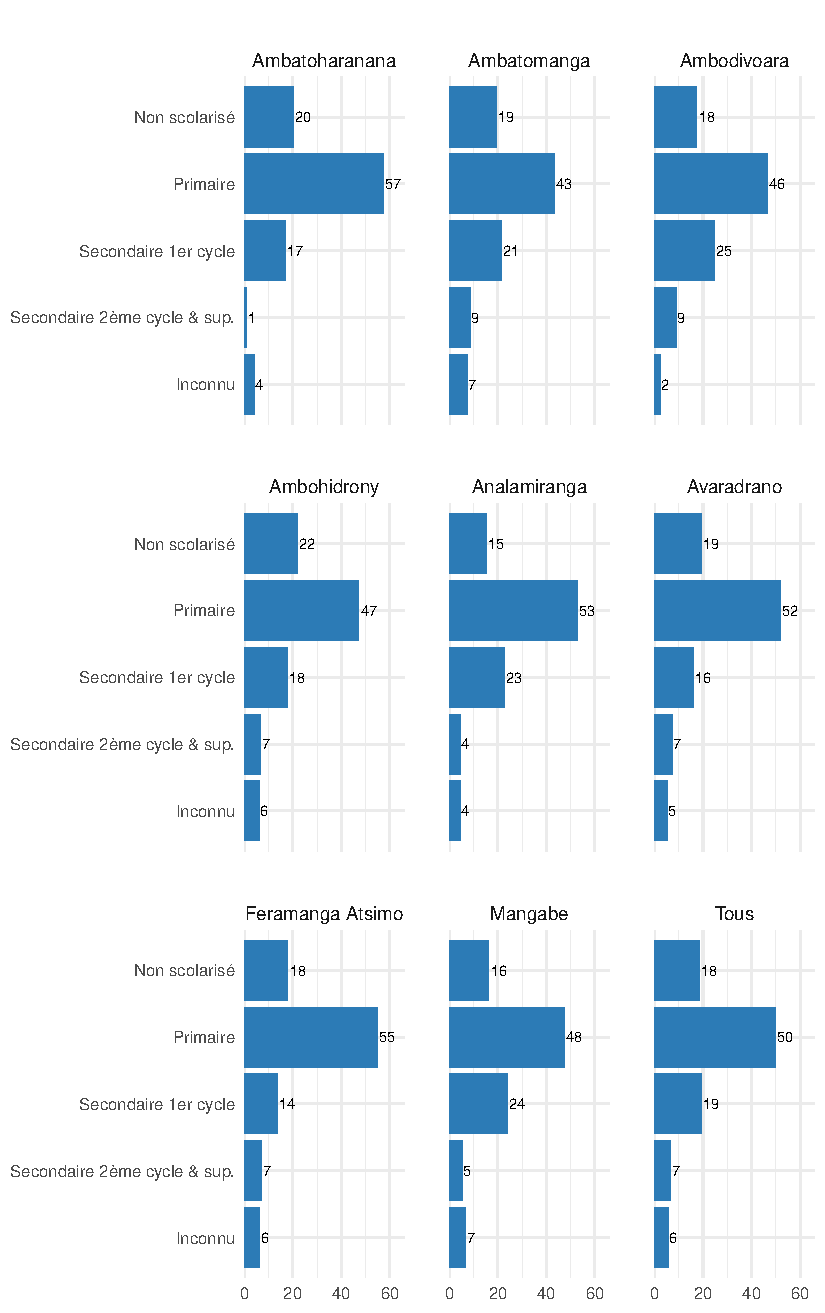
\includegraphics[keepaspectratio]{02_structure_menages_files/figure-pdf/fig_other_educ-1.pdf}}

}

\end{figure}%

\subsubsection{Niveau d'éducation des autres membres par
sexe}\label{niveau-duxe9ducation-des-autres-membres-par-sexe}

À Marovoay, le niveau primaire est atteint par 49.8 \% des femmes et
45.6 \% des membres masculins. La disparité de genre est
particulièrement visible dans l'accès au premier cycle du secondaire qui
touche 17.1 \% des femmes contre seulement 10.4 \% des hommes. Pour les
niveaux d'études les plus élevés (second cycle et supérieur), les taux
sont plus faibles et relativement proches entre les sexes avec 6.1 \%
pour les femmes et 6.7 \% pour les hommes. In fine, les femmes affichent
également une meilleure insertion scolaire initiale avec 24.4 \% de
personnes non scolarisées contre 31.8 \% pour les hommes.

\begin{figure}[H]

\caption{Niveau d'éducation des autres membres par sexe}

{\centering \pandocbounded{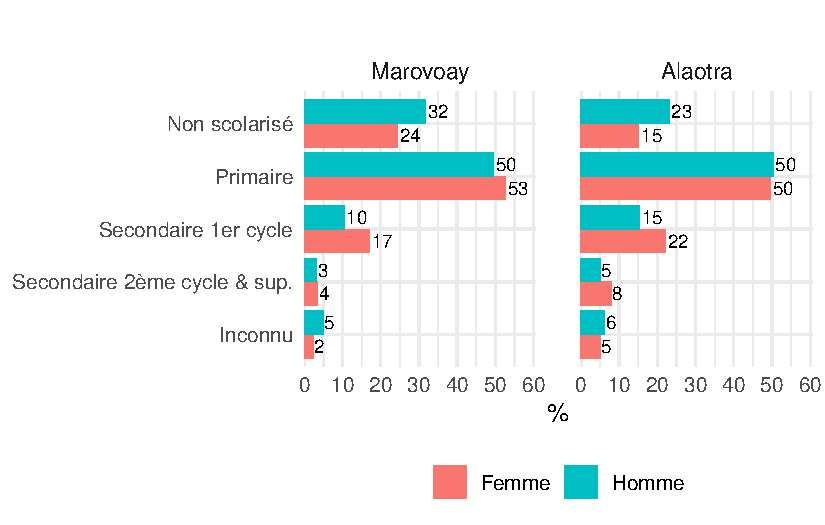
\includegraphics[keepaspectratio]{02_structure_menages_files/figure-pdf/fig_other_educ_sex-1.pdf}}

}

\end{figure}%

\subsubsection{Alphabétisation des autres
membres}\label{alphabuxe9tisation-des-autres-membres}

Cette section analyse les capacités de lecture et d'écriture des membres
du ménage autres que le CM fournissant un indicateur de la qualité du
capital humain au sein des familles rurales. L'évaluation distingue les
personnes capables de lire ou d'écrire aisément de celles qui le font
avec effort ou qui en sont incapables.

\paragraph{Savoir lire}\label{savoir-lire-1}

À Marovoay, l'aptitude à la lecture est globalement moins répandue. La
tendance en faveur des femmes persiste avec 59.3 \% lisant sans
difficulté contre 52.9 \% pour les hommes. Cependant, 13.9 \% des femmes
et 16.9 \% des hommes déclarent lire avec effort. Enfin, le taux de
membres ne sachant pas lire du tout s'élève à 26.9 \% chez les femmes et
atteint 30.1 \% chez les hommes.

\begin{figure}[H]

\caption{Aptitude à la lecture des autres membres selon le sexe}

{\centering \pandocbounded{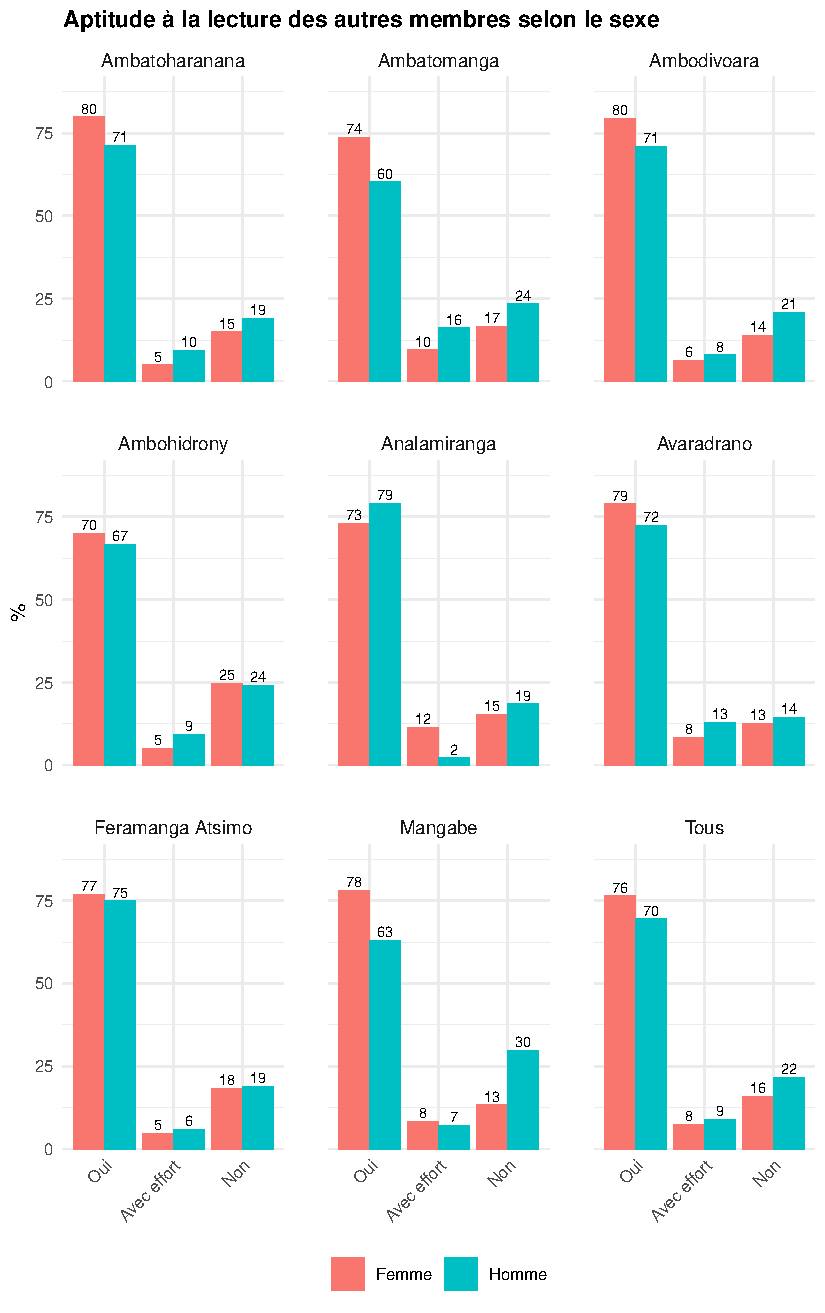
\includegraphics[keepaspectratio]{02_structure_menages_files/figure-pdf/fig_other_read_sex-1.pdf}}

}

\end{figure}%

\paragraph{Savoir écrire}\label{savoir-uxe9crire-1}

À Marovoay, le niveau de compétence en écriture est sensiblement plus
bas avec 56.8 \% des membres capables d'écrire aisément. Les difficultés
y sont plus marquées avec 15.0 \% des personnes écrivant avec effort et
28.3 \% déclarant ne pas savoir écrire du tout.

À Marovoay, l'aptitude à l'écriture est globalement moins répandue.
Cependant, la tendance en faveur des femmes persiste avec 59.2 \%
écrivant sans difficulté contre 53.0 \% pour les hommes. Les difficultés
à l'écrit sont marquées pour les deux sexes avec 13.6 \% des femmes et
17.1 \% des hommes déclarant écrire avec effort. Le taux de personnes ne
possédant aucune compétence en écriture est élevé dans cet observatoire
s'élevant à 27.3 \% chez les femmes et atteignant 29.9 \% chez les
hommes.

\begin{figure}[H]

\caption{Aptitude à l'écriture des autres membres selon le sexe}

{\centering \pandocbounded{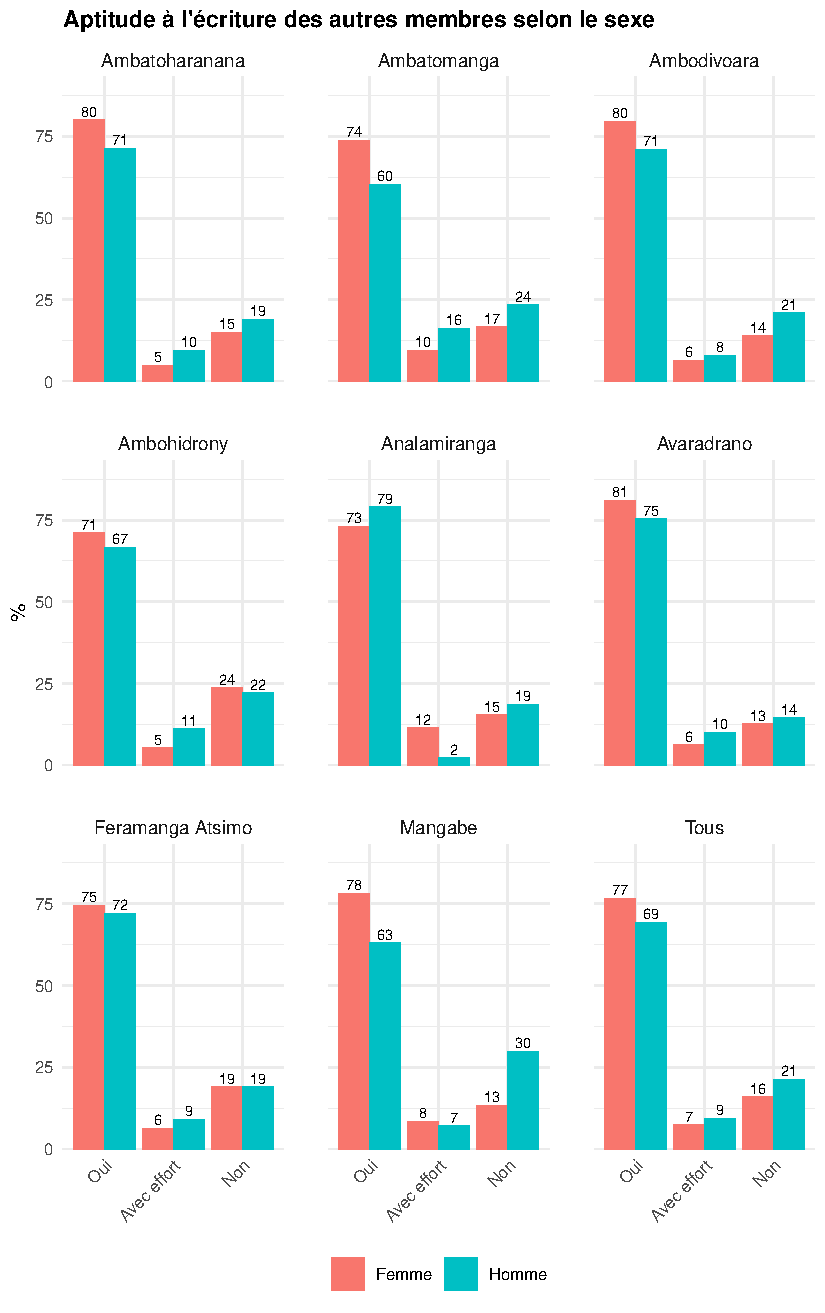
\includegraphics[keepaspectratio]{02_structure_menages_files/figure-pdf/fig_other_write_sex-1.pdf}}

}

\end{figure}%

\subsection{Scolarisation}\label{scolarisation}

Le taux de scolarisation des enfants de 6 à 14 ans constitue un
indicateur clé du développement humain et de l'investissement des
ménages dans l'éducation.

\subsubsection{Taux net de scolarisation des enfants de 6 à 14
ans}\label{taux-net-de-scolarisation-des-enfants-de-6-uxe0-14-ans}

Dans Marovoay, le taux net de scolarisation s'élève à 81.7 \%.

La progression scolaire suit globalement la structure attendue par âge.
Entre 3 et 5 ans, les enfants sont majoritairement en préscolaire, avec
une part déjà entrée en CP1. Chez les 6-10 ans, les classes du primaire
dominent nettement, en particulier le CP2, le CE et le CM1-CM2. Entre 11
et 14 ans, la répartition se déplace vers la fin du primaire et le
premier cycle du secondaire, surtout la 6e et la 5e. Enfin, les 15-17
ans se concentrent davantage dans les classes du secondaire, tandis que
les niveaux supérieurs n'apparaissent que parmi les 18-25 ans.

\subsubsection{Raisons de non fréquentation de l'école pour les 6 à 15
ans}\label{raisons-de-non-fruxe9quentation-de-luxe9cole-pour-les-6-uxe0-15-ans}

La Figure~\ref{fig-raisons-non-scol} détaille l'ensemble des motifs de
non-scolarisation cités.

A Marovoay, parmi les enfants de 6 à 15 ans non scolarisés, la première
raison invoquée est « Frais trop élevés » (52.1 \%).

\begin{figure}

\caption{\label{fig-raisons-non-scol}Principales raisons de
non-scolarisation ou d'arrêt des études (6-15 ans)}

\centering{

\pandocbounded{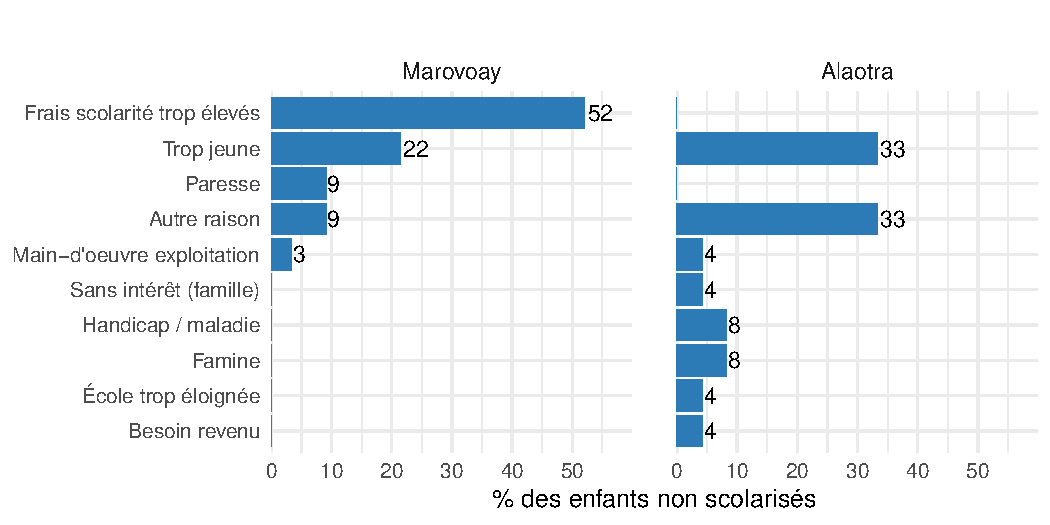
\includegraphics[keepaspectratio]{02_structure_menages_files/figure-pdf/fig-raisons-non-scol-1.pdf}}

}

\end{figure}%

\subsection{Activités principales des autres membres de
ménages}\label{activituxe9s-principales-des-autres-membres-de-muxe9nages}

La répartition sectorielle des activités des autres membres de ménage
reflète la diversification économique au sein des familles et le rôle
des conjoints et enfants dans l'économie du ménage. Les activités sont
regroupées selon la même nomenclature sectorielle que pour les CM.

A Marovoay, les cultivateurs exploitants constituent également
l'activité principale la plus fréquente avec 49 \%. Les ouvriers
agricoles représentent 17 \% des autres membres. Les activités restantes
occupent des parts plus faibles, avec 9 \% pour les élèves et étudiants
ainsi que pour les inactifs et retraités, 8 \% pour le commerce et la
restauration, 4 \% pour l'artisanat, le BTP et le transport, puis 2 \%
chacun pour les services et autres activités ainsi que pour l'élevage,
la pêche et les ressources naturelles.

\begin{figure}

\caption{\label{fig-other-act}}

\centering{

\pandocbounded{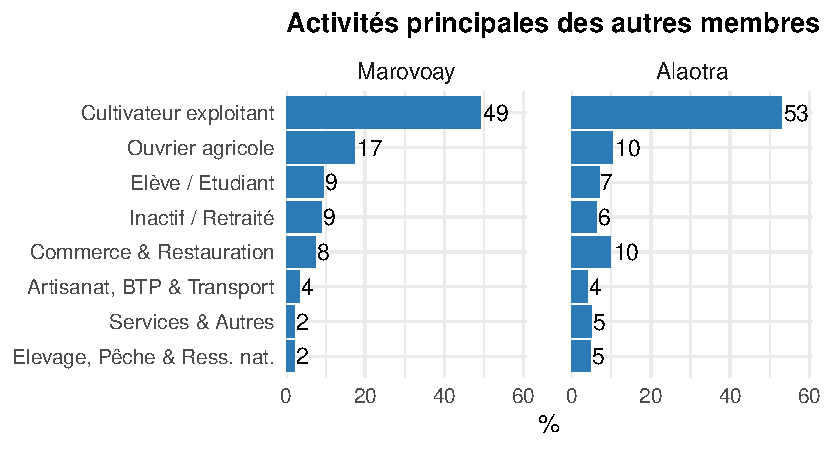
\includegraphics[keepaspectratio]{02_structure_menages_files/figure-pdf/fig-other-act-1.pdf}}

}

\end{figure}%

\subsubsection{Activités principales des autres membres par
sexe}\label{activituxe9s-principales-des-autres-membres-par-sexe}

À Marovoay, la fonction de cultivateur exploitant est également
prédominante, surtout chez les femmes qui sont 53.5 \% contre 39.1 \%
pour les hommes. Le recours au salariat agricole est plus intense qu'à
l'Alaotra, avec 18.6 \% d'hommes et 16.7 \% de femmes travaillant comme
ouvriers agricoles. Une disparité majeure apparaît dans le statut
d'élève ou étudiant, qui concerne 17.8 \% des membres masculins mais
seulement 5.7 \% des membres féminins. Le secteur des services et autres
activités emploie 14.3 \% des hommes et 9.6 \% des femmes. Le commerce
et la restauration restent portés par les femmes avec un taux de 10.1 \%
contre moins de 5 \% pour les hommes. Les secteurs de l'artisanat, du
BTP et du transport occupent 5.4 \% des hommes et 2.7 \% des femmes.
Enfin, l'élevage, la pêche et l'exploitation des ressources naturelles
concernent 3.1 \% des hommes et 1.7 \% des membres féminins.

\pandocbounded{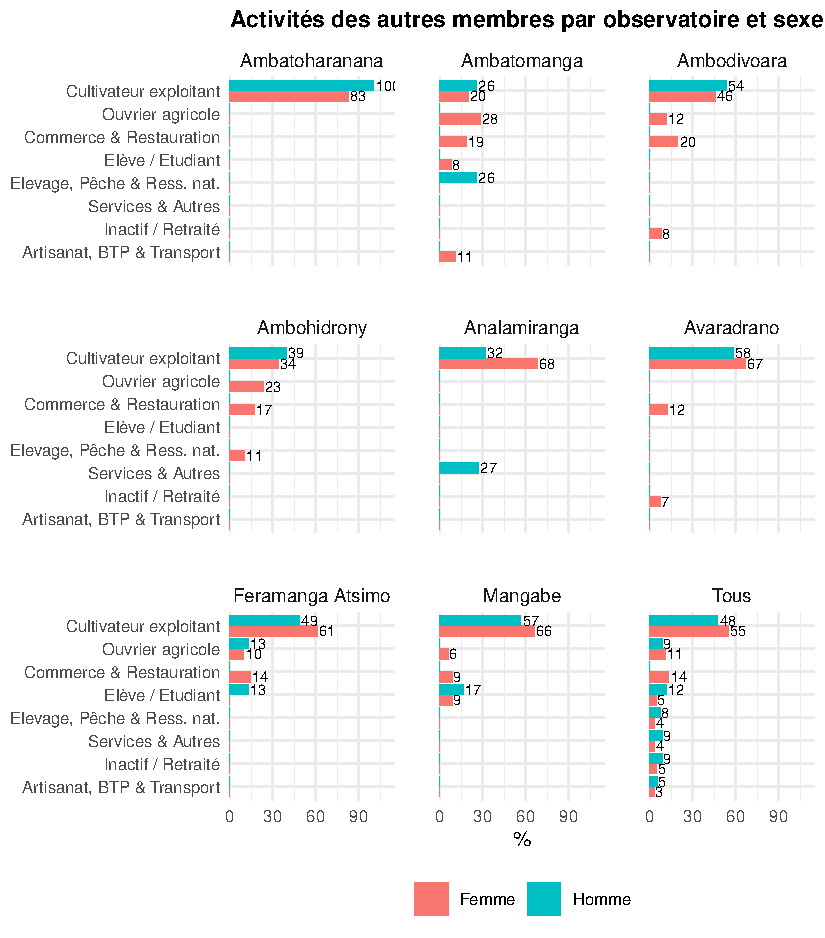
\includegraphics[keepaspectratio]{02_structure_menages_files/figure-pdf/fig_other_act_sex-1.pdf}}

\bookmarksetup{startatroot}

\chapter{Habitat et niveau de vie}\label{habitat-et-niveau-de-vie}

Cette section decrit les conditions d'habitat, les equipements des
menages, leurs transferts et revenus.

À Marovoay, les conditions d'habitat sont étroitement liées à la
position des ménages par rapport au fleuve Betsiboka. Les fokontany de
la rive droite (Bepako, Madiromiongana), situés en lisière du Parc
national d'Ankarafantsika, ont un accès plus limité aux ressources en
bois et matériaux de construction, notamment en raison des restrictions
liées à la conservation. L'approvisionnement en eau dépend en grande
partie du fleuve et de puits traditionnels. L'équipement agricole y est
dominé par les outils manuels, complétés par le recours à la traction
bovine pour le labour des rizières.

\section{Habitat}\label{habitat}

Les conditions d'habitat des ménages enquêtés témoignent des réalités du
milieu rural malgache. Le statut d'occupation, le type d'assainissement,
l'accès à l'eau, le mode d'éclairage et la source d'énergie de cuisson
constituent des indicateurs essentiels du cadre de vie.

\subsection{Statut d'occupation du
logement}\label{statut-doccupation-du-logement}

Le statut d'occupation du logement traduit la sécurité résidentielle des
ménages.

À Marovoay, 88.1 \% des ménages occupent un logement en « En propriété
», avec des proportions particulièrement élevées dans les localités les
plus enclavées. À l'inverse, la location reste plus présente dans les
hameaux proches de l'axe routier. Ces disparités traduisent des niveaux
différents de sécurité résidentielle selon le positionnement
géographique des ménages.

\begin{figure}

\caption{\label{fig-statut-logement}Statut d'occupation du logement}

\centering{

\pandocbounded{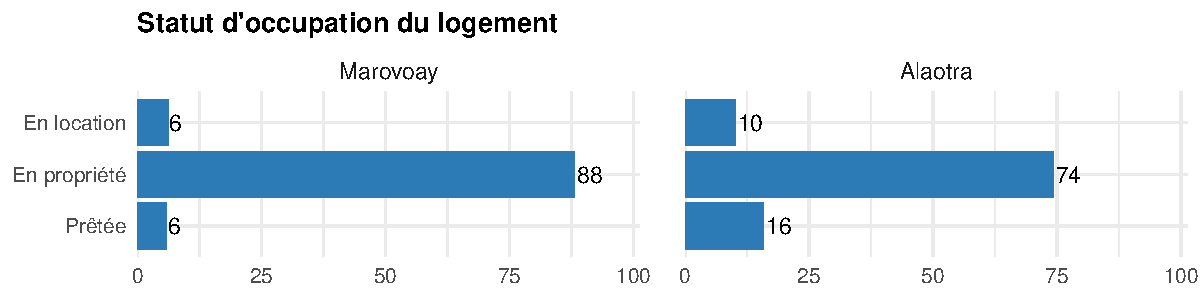
\includegraphics[keepaspectratio]{03_habitat_niveau_de_vie_files/figure-pdf/fig-statut-logement-1.pdf}}

}

\end{figure}%

\subsection{Type de latrine}\label{type-de-latrine}

Le type de latrine constitue un indicateur sanitaire fondamental.

À Marovoay, le type dominant est « Dans la nature » (48.2 \% des
ménages). L'assainissement se caractérise par une forte prévalence de la
défécation à l'air libre et une utilisation limitée des latrines
améliorées. Les fosses perdues en commun et les fosses perdues
individuelles occupent une place secondaire, chacune étant utilisée par
un quart des ménages. De nettes disparités territoriales existent entre
les localités, les hameaux les plus éloignés présentant les taux d'accès
les plus faibles aux infrastructures sanitaires.

\begin{figure}

\caption{\label{fig-latrine}Types de latrine}

\centering{

\pandocbounded{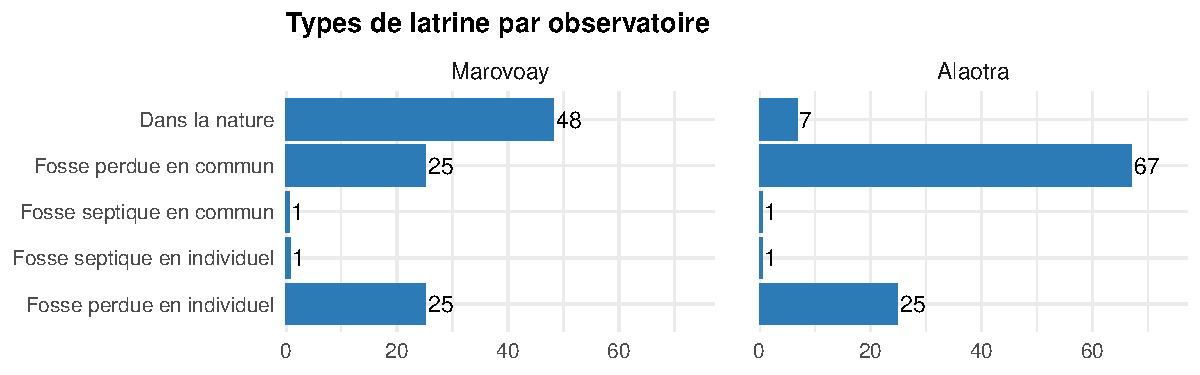
\includegraphics[keepaspectratio]{03_habitat_niveau_de_vie_files/figure-pdf/fig-latrine-1.pdf}}

}

\end{figure}%

\subsection{Accès a l'eau}\label{accuxe8s-a-leau}

L'approvisionnement en eau détermine en grande partie les conditions
sanitaires des ménages ruraux. L'accès à une eau plus sécurisée est
nettement supérieur à Alaotra. Marovoay reste très dépendant des eaux de
surface prenant source au fleuve Betsiboka. Ce qui pose des enjeux de
santé publique.

À Marovoay, l'approvisionnement en eau repose principalement sur les «
Cours d?eau » utilisés par 37.4 \% des ménages. . Les ménages dépendent
fortement des sources naturelles : cours d'eau et puits non aménagés
représentent ensemble une part importante de l'approvisionnement
(27.6\%).L'accès à l'eau améliorée (bornes fontaines publiques, eau
courante) reste limité à l'échelle de l'observatoire, avec des
disparités marquées entre localités. Les puits à margelle représentent
aussi une part notable avec 11.2\% des ménages utilisateurs.

\begin{figure}

\caption{\label{fig-eau}Mode d'approvisionnement en eau}

\centering{

\pandocbounded{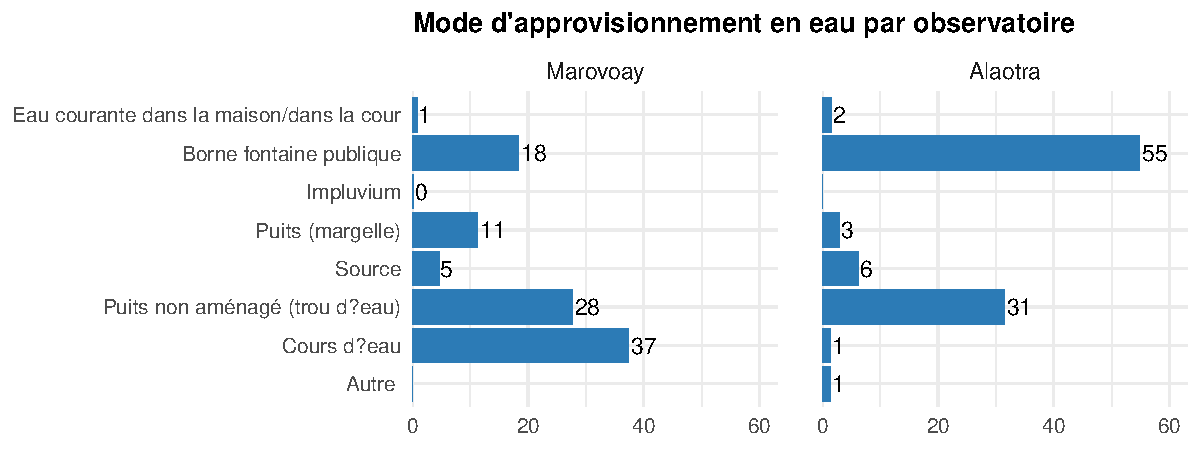
\includegraphics[keepaspectratio]{03_habitat_niveau_de_vie_files/figure-pdf/fig-eau-1.pdf}}

}

\end{figure}%

\subsection{Mode d'éclairage}\label{mode-duxe9clairage}

Le mode d'éclairage reflète le niveau d'accès à l'énergie moderne. Les
ménages ruraux dépendent encore largement de sources traditionnelles,
même si la pénétration du solaire progresse.

À Marovoay, le pétrole lampant constitue également le principal mode
d'éclairage, avec 54.5\% des ménages concernés. L'énergie solaire
représente le deuxième mode d'éclairage le plus utilisé avec 31.2\%,
suivie des piles qui concernent 29.1\% des ménages. Les batteries sont
aussi utilisées par une part non négligeable des ménages, soit 12.5\%.

Enfin, le recours au bois de chauffe comme mode d'éclairage reste
marginal dans les deux observatoires.

\begin{figure}

\caption{\label{fig-eclairage}Modes d'éclairage}

\centering{

\pandocbounded{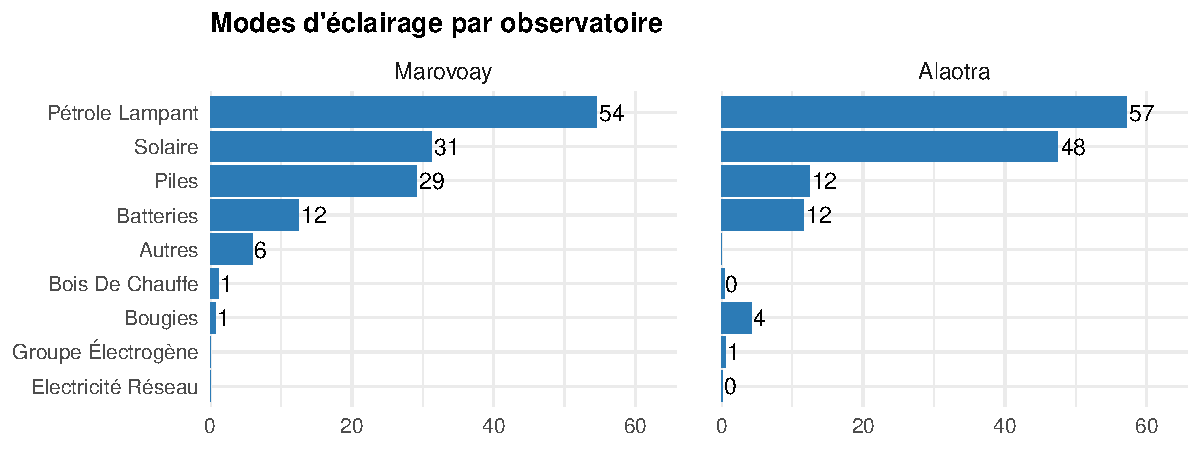
\includegraphics[keepaspectratio]{03_habitat_niveau_de_vie_files/figure-pdf/fig-eclairage-1.pdf}}

}

\end{figure}%

À Marovoay, la situation est similaire, avec 92\% des utilisateurs de
l'énergie solaire possédant des panneaux en état de marche. À l'inverse,
8\% des ménages utilisateurs indiquent que leurs panneaux solaires ne
sont pas fonctionnels.

Parmi les ménages utilisant le solaire, la proportion disposant d'un
panneau en état de marche est présentée ci-dessous.

\subsection{Source d'énergie pour la
cuisson}\label{source-duxe9nergie-pour-la-cuisson}

La quasi-totalité des ménages ruraux malgaches dépendent de la biomasse
pour la cuisson. La nature exacte du combustible utilisé (bois, charbon
de bois) varie selon la disponibilité locale des ressources forestières.

À Marovoay, le bois de chauffe demeure également le mode de cuisson
dominant, concernant 72.6\% des ménages. Le charbon est aussi largement
utilisé, avec 46.4\% des ménages qui y recourent. Les autres modes de
cuisson apparaissent quant à eux très peu utilisés dans cet
observatoire.

\begin{figure}

\caption{\label{fig-cooking}}

\centering{

\pandocbounded{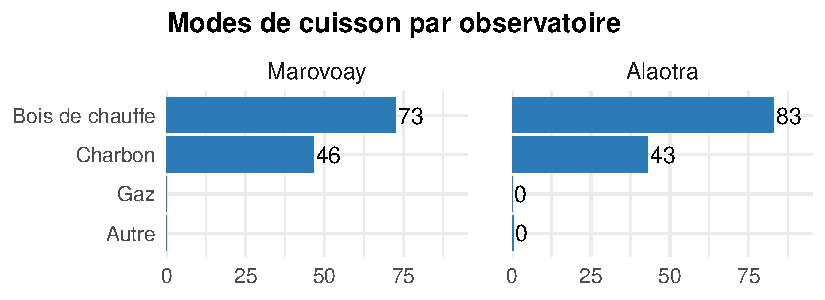
\includegraphics[keepaspectratio]{03_habitat_niveau_de_vie_files/figure-pdf/fig-cooking-1.pdf}}

}

\end{figure}%

\section{Niveau de vie}\label{niveau-de-vie}

La possession de biens durables constitue un proxy classique du niveau
de vie des ménages en milieu rural, où les revenus monétaires sont
souvent difficiles à mesurer.

\subsection{Biens de confort courant}\label{biens-de-confort-courant}

Les biens de confort courant (mobilier, ustensiles, outils) renseignent
sur le niveau d'équipement quotidien des ménages et constituent un
indicateur de bien-être matériel.

À Marovoay, les marmites constituent également le bien de confort le
plus courant, suivies des nattes pour dormir qui concernent 83.2\% des
ménages. Les téléphones fixes ou mobiles sont présents dans 69\% des
ménages, tandis que les tables et les lits concernent respectivement
64.4\% et 63.4\% des ménages. La radio ou le radio-K7 reste aussi
relativement répandue avec 47.6\%. Les autres équipements, notamment la
bicyclette, la télévision, la moto, le lecteur VCD/DVD, l'antenne
parabolique et la voiture, restent faiblement représentés.

\begin{figure}

\caption{\label{fig-comfort}}

\centering{

\pandocbounded{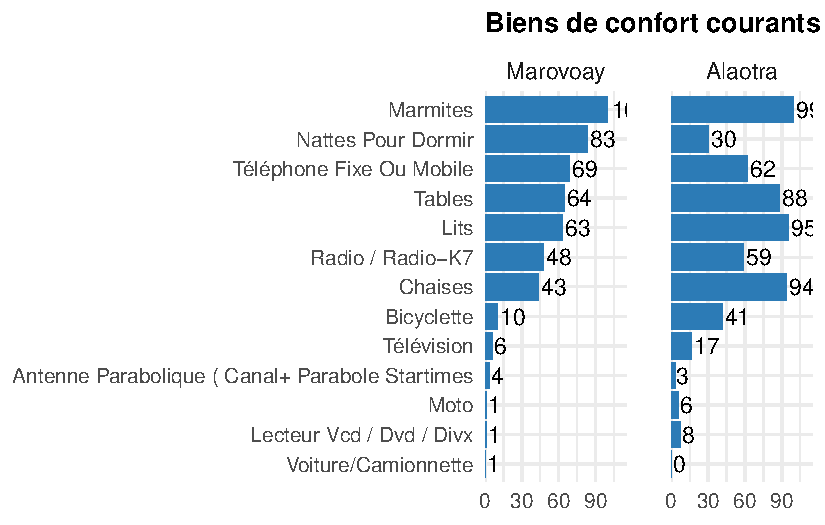
\includegraphics[keepaspectratio]{03_habitat_niveau_de_vie_files/figure-pdf/fig-comfort-1.pdf}}

}

\end{figure}%

\subsection{Equipement agricole}\label{equipement-agricole}

L'équipement agricole conditionne la productivité et la capacité
d'extension des surfaces cultivées. La possession de matériel mécanisé
ou de traction animale constitue un facteur de différenciation important
entre les ménages.

À Marovoay, l'angady constitue également l'équipement agricole dominant
avec 81.9\% des ménages concernés, suivi de la faucille ou coupe-coupe
utilisée par 60.5\% des ménages. Les haches, les charrues et les
couteaux occupent aussi une place notable, avec respectivement 25.6\%,
23.5\% et 22\% des ménages utilisateurs. Les herses, pulvériseurs et
rotovators concernent 20.2\% des ménages. Les autres équipements
agricoles notamment la charette attelée, la sarcleuse, la pompe
hydraulique ou le motoculteur du type Kubota, et le tracteur demeurent
peu répandus dans cet observatoire.

\begin{figure}

\caption{\label{fig-table-equip}}

\centering{

\pandocbounded{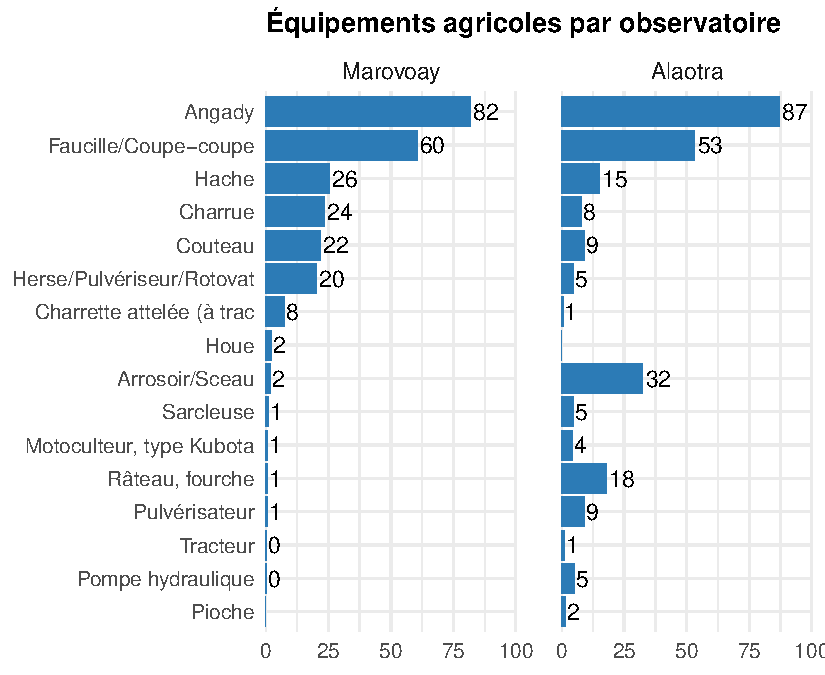
\includegraphics[keepaspectratio]{03_habitat_niveau_de_vie_files/figure-pdf/fig-table-equip-1.pdf}}

}

\end{figure}%

\subsection{Matériel de communication audiovisuelle et
télécommunication}\label{matuxe9riel-de-communication-audiovisuelle-et-tuxe9luxe9communication}

L'accès aux technologies de communication et d'information constitue un
vecteur de connexion aux marchés, aux services et à l'information. La
pénétration du téléphone mobile a transformé les pratiques économiques
et sociales en milieu rural.

A Marovoay, la radio domine aussi avec 44\%, suivie de près par le
téléphone fixe ou mobile à 41\%. La télévision est beaucoup moins
répandue, ne représentant que 5.3\%. Les lecteurs VCD, DVD ou DivX sont
quasi absents avec seulement 1\%, et l'antenne parabolique atteint
3.1\%. Ces données révèlent une forte dépendance aux outils de
communication de base avec une présence très réduite des équipements
audiovisuels modernes.

\begin{figure}

\caption{\label{fig-comm}}

\centering{

\pandocbounded{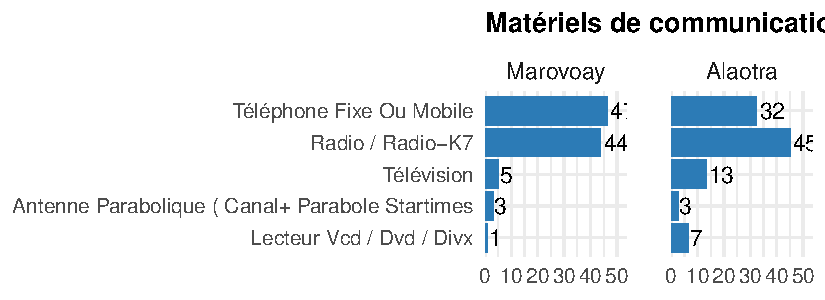
\includegraphics[keepaspectratio]{03_habitat_niveau_de_vie_files/figure-pdf/fig-comm-1.pdf}}

}

\end{figure}%

\section{Transferts sortants}\label{transferts-sortants}

La section consacrée aux transferts sortants recense les aides envoyées
par les ménages à des personnes extérieures au foyer, en précisant
notamment le type de transfert (argent ou riz), sa valeur et le lieu de
résidence du destinataire.

À Marovoay, la part des ménages envoyeurs est de 13,7 \%. Les transferts
en riz présentent une valeur moyenne de 335 000 Ar, tandis que les
transferts en argent enregistrent une valeur moyenne de 86 000 Ar.

\begin{figure}

\caption{\label{fig-transferts-sortants}Valeur moyenne des transferts
sortants par observatoire et type}

\centering{

\pandocbounded{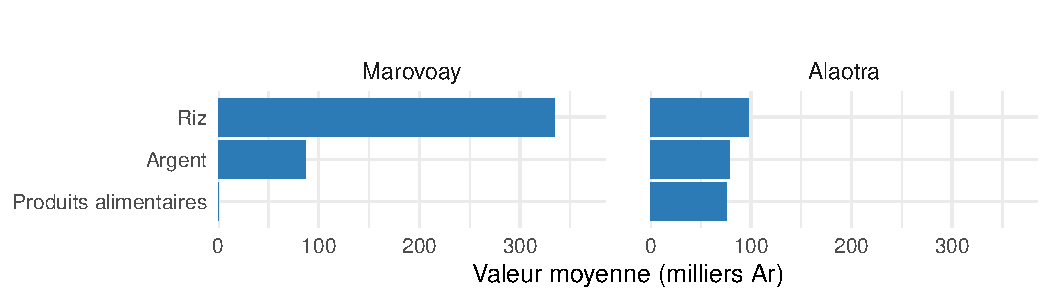
\includegraphics[keepaspectratio]{03_habitat_niveau_de_vie_files/figure-pdf/fig-transferts-sortants-1.pdf}}

}

\end{figure}%

À Marovoay, la part des ménages envoyeurs est plus faible, s'élevant à
13,7 \% de l'échantillon.

\begin{table}

\caption{\label{tbl-transferts-sortants}Transferts sortants : resume par
observatoire}

\centering{

}

\end{table}%

À Marovoay, 77,1 \% des transferts sont destinés à des personnes vivant
dans la même commune. Ceux installés dans une autre commune de la même
région représentent 10,8 \%, et les transferts vers une autre région
atteignent 12,0 \%.

\begin{figure}

\caption{\label{fig-destination-transferts}Lieu de residence des
destinataires de transferts}

\centering{

\pandocbounded{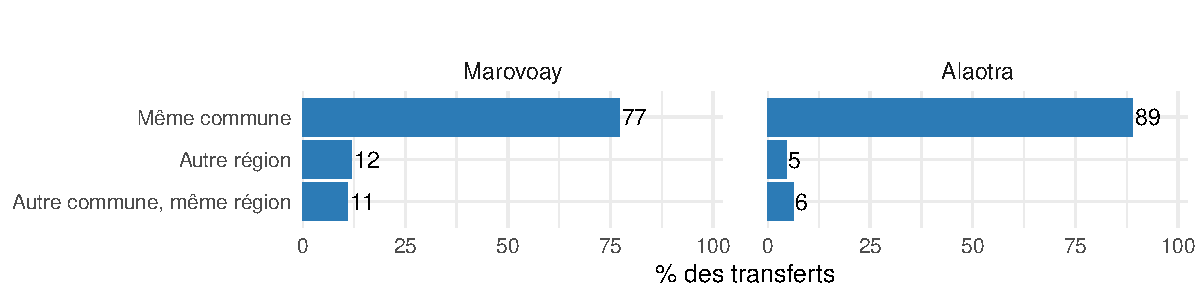
\includegraphics[keepaspectratio]{03_habitat_niveau_de_vie_files/figure-pdf/fig-destination-transferts-1.pdf}}

}

\end{figure}%

\section{Revenu}\label{revenu}

L'analyse des revenus constitue un élément essentiel dans l'étude des
conditions de vie des ménages ruraux. Elle permet d'apprécier leur
capacité à satisfaire les besoins fondamentaux et à faire face aux
différentes contraintes économiques. L'étude des sources et du niveau
des revenus offre également une meilleure compréhension des stratégies
de subsistance adoptées par les ménages en milieu rural.

Les revenus présentés ici sont des revenus annuels par ménage, calculés
sur la période de référence (PR) de la campagne 2025. Le revenu total se
décompose en revenu courant et revenu exceptionnel.

Le revenu courant agrège sept composantes :

\begin{itemize}
\tightlist
\item
  les \textbf{salaires agricoles} : rémunération du travail salarié
  agricole ;
\item
  les \textbf{salaires non-agricoles} : rémunération du travail salarié
  hors agriculture ;
\item
  les \textbf{revenus indépendants} : revenus des activités libérales et
  artisanales non-agricoles ;
\item
  le \textbf{revenu net rizicole}: valeur de la production de riz moins
  les charges ;
\item
  le \textbf{revenu net des autres cultures} : même logique pour les
  cultures non-rizicoles ;
\item
  le \textbf{revenu de l'élevage} : ventes d'animaux (autre que les
  animaux considérés comme capitaux comme les bœufs de trait etc\ldots)
  et produits d'élevage ;
\item
  et la \textbf{pêche}.
\end{itemize}

Le revenu exceptionnel regroupe les rentes foncières, les autres
revenus, le travail HIMO, la décapitalisation (y compris la vente des
animaux considérés comme capitaux) et les transferts reçus.

\subsection{Structure du revenu total}\label{structure-du-revenu-total}

Le revenu total annuel par ménage synthétise l'ensemble des ressources
monétaires et non-monétaires. Les écarts entre moyenne et médiane
reflètent le degré d'inégalité au sein de chaque observatoire.

Afin de mieux apprécier le niveau de vie, le revenu total est également
rapporté à la taille du ménage. On distingue le revenu « par tête »
(revenu total divisé par le nombre de membres) et le revenu « par unité
de consommation » (UC). Pour ce dernier, nous utilisons l'échelle
d'équivalence de l'OCDE modifiée, qui attribue un poids de 1,0 au
premier adulte, 0,5 aux autres personnes de 14 ans ou plus, et 0,3 aux
enfants de moins de 14 ans. Cette méthode permet de tenir compte des
économies d'échelle au sein du ménage (partage du logement, de
l'énergie, etc.).

À Marovoay, le revenu annuel moyen par ménage est de 3 480 646 Ar et la
médiane est de 2 094 749 Ar. L'écart-type est de 5 475 598 Ar indiquant
une variation importante des revenus au sein des ménages enquêtés.
Chaque individu dispose en moyenne d'un revenu annuel de 870.716 Ar,
soit environ 72.560 Ar par mois. Après ajustement selon l'échelle
d'équivalence de l'OCDE modifiée, le revenu annuel moyen atteint
1.473.963 Ar par unité de consommation, soit environ 122.830 Ar par
mois.

\subsection{Decomposition du revenu
courant}\label{decomposition-du-revenu-courant}

La décomposition du revenu courant en ses sept composantes met en
lumière la structure productive de chaque observatoire et le degré de
dépendance à l'égard de la riziculture.

A Marovoay, les revenus nets rizicoles représentent la plus grande part
du revenu courant moyen par ménage avec 39.2 \% du total, soit 1 287 310
Ar/an. Les revenus indépendants se placent en deuxième position avec
23.2 \%, correspondant à 759 874 Ar/an. Les salaires agricoles arrivent
ensuite avec 18.4 \%, soit 604 846 Ar/an. L'élevage contribue pour 7.7
\% du revenu courant moyen, représentant 253 697 Ar/an. Les salaires non
agricoles participent à hauteur de 6.2 \%, soit 204 131 Ar/an. Les
revenus nets des autres cultures représentent 5.2 \%, correspondant à
170 901 Ar/an. Le revenu courant moyen total par ménage dans
l'observatoire de Marovoay est de 3 280 758 Ar/an.

Pour les deux observatoires, la pêche ne contribue pas au revenu courant
moyen.

\begin{figure}[H]

\caption{Part des composantes dans le revenu courant moyen par
observatoire}

{\centering \pandocbounded{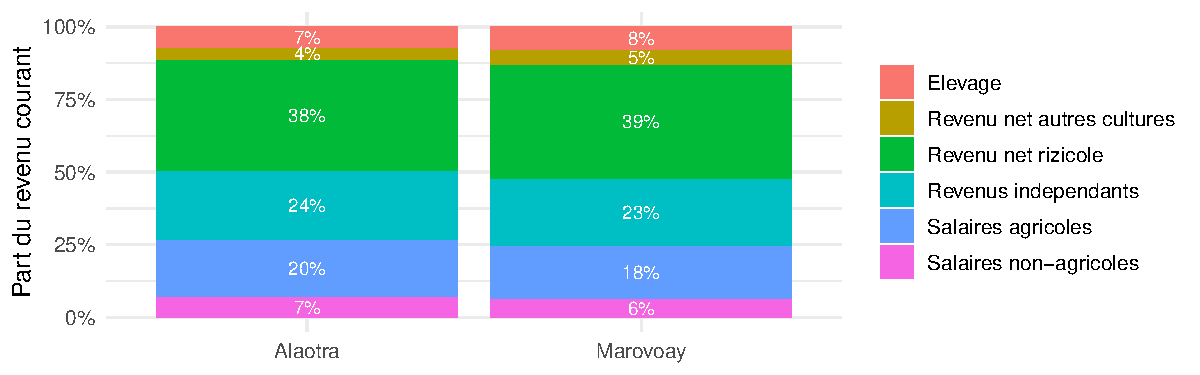
\includegraphics[keepaspectratio]{03_habitat_niveau_de_vie_files/figure-pdf/fig_revcou_shares-1.pdf}}

}

\end{figure}%

\subsection{Distribution du revenu
total}\label{distribution-du-revenu-total}

La distribution du revenu total illustre le degré d'inégalité au sein de
chaque observatoire. L'utilisation d'une échelle logarithmique permet de
mieux visualiser l'étalement de la distribution et la concentration des
ménages à bas revenus.

Afin de mieux apprécier le niveau de vie, le revenu total est également
rapporté à la taille du ménage. On distingue le revenu « par tête »
(revenu total divisé par le nombre de membres) et le revenu « par unité
de consommation » (UC). Pour ce dernier, nous utilisons l'échelle
d'équivalence de l'OCDE modifiée, qui attribue un poids de 1,0 au
premier adulte, 0,5 aux autres personnes de 14 ans ou plus, et 0,3 aux
enfants de moins de 14 ans. Cette méthode permet de tenir compte des
économies d'échelle au sein du ménage (partage du logement, de
l'énergie, etc.).




\end{document}
